% !TeX encoding = UTF-8
% !TeX program = pdflatex
% !TeX spellcheck = en_US

% https://biccari.altervista.org/c/informatica/latex/sapthesis.php

\documentclass[LaM,binding=0.6cm]{sapthesis}

\usepackage{microtype}

\usepackage{hyperref}
\usepackage[noabbrev,capitalize]{cleveref}
\usepackage{amsfonts}
\usepackage[square, authoryear]{natbib}
\usepackage{setspace}
\usepackage{subcaption}

\onehalfspacing
%\doublespacing

\crefformat{section}{\S#2#1#3} % see manual of cleveref, section 8.2.1
\crefformat{subsection}{\S#2#1#3}
\crefformat{subsubsection}{\S#2#1#3}

\hypersetup{pdftitle={Cycle-Consistent Story Generation},pdfauthor={Amr Fathy}}

\newcommand{\bs}{\textbackslash}

% Commands for the titlepage
\title{Cycle-Consistent Story Generation}
\author{Amr Fathy}
\IDnumber{1848399}
\course{Artificial Intelligence and Robotics}
\courseorganizer{Dipartimento di Ingegneria Informatica, Automatica e Gestionale}
\AcademicYear{2020/2021}
\copyyear{2021}
\advisor{Prof. Roberto Navigli}
\coadvisor{Dr. Rexhina Blloshmi}
\authoremail{amru.a.fathy@gmail.com}

\examdate{October 22, 2021}
\examiner{Prof.  Marco Schaerf}
\examiner{Prof. Anagnostopoulos Aristidis}
\examiner{Prof. Daniele Nardi}
\examiner{Prof. Roberto Navigli}
\examiner{Prof. Fiora Pirri}
\examiner{Prof. Marilena Vendittelli}
\examiner{Prof. Daniele Venturi}
\versiondate{\today}


\begin{document}

\frontmatter

\maketitle

%\dedication{Dedicated to\\ Donald Knuth}

\addcontentsline{toc}{chapter}{Abstract}

\begin{abstract}

% https://www.ldeo.columbia.edu/~martins/sen_sem/thesis_org.html


Even though we are currently experiencing a technological revolution, with virtual assistants becoming a vital part of it, many of these agents are still lacking when it comes to proper communication. Humans are natural storytellers, thus it is fitting that these Artificial Intelligence-powered agents are able to properly understand and tell stories.

Automated story generation is a field of AI where the goal is to create agents that tell \textit{good} stories. A story being good is subjective and hard to define. In this thesis, we will discuss and deal with some well-defined metrics to measure the quality of generated stories.

Previous methods relied on symbolic planning and knowledge databases to generate stories, which made them domain-rigid and limitedly coherent. Recently, neural-based approaches have shown more promise in terms of the quality of generated stories and their ability to reduce the need for knowledge databases. Nevertheless, these systems still lack originality, long-term coherence, and other problems.

In this study, we try to improve story generation by leveraging the knowledge of large pretrained models and utilizing extra training signals through a cycle-consistency framework. More formally, we exploit the dual tasks of text generation and summarization as means to improve the performance of the story generation task. We show that the cycle-consistency framework offers better results in text overlap and text diversity metrics.

\end{abstract}


%\begin{acknowledgments}
\end{acknowledgments}


\tableofcontents
%\listoffigures
%\listoftables

% Do not use the starred version of the chapter command!

\mainmatter

\chapter{Introduction}
\label{ch:introduction}

%You can't write a good introduction until you know what the body of the paper says. Consider writing the introductory section(s) after you have completed the rest of the paper, rather than before.
%Be sure to include a hook at the beginning of the introduction. This is a statement of something sufficiently interesting to motivate your reader to read the rest of the paper, it is an important/interesting scientific problem that your paper either solves or addresses. You should draw the reader in and make them want to read the rest of the paper.

%The next paragraphs in the introduction should cite previous research in this area. It should cite those who had the idea or ideas first, and should also cite those who have done the most recent and relevant work. You should then go on to explain why more work was necessary (your work, of course.)
 
%What else belongs in the introductory section(s) of your paper? 
%A statement of the goal of the paper: why the study was undertaken, or why the paper was written. Do not repeat the abstract. 
%Sufficient background information to allow the reader to understand the context and significance of the question you are trying to address. 
%Proper acknowledgement of the previous work on which you are building. Sufficient references such that a reader could, by going to the library, achieve a sophisticated understanding of the context and significance of the question.
%The introduction should be focused on the thesis question(s).  All cited work should be directly relevent to the goals of the thesis.  This is not a place to summarize everything you have ever read on a subject.
%Explain the scope of your work, what will and will not be included. 
%A verbal "road map" or verbal "table of contents" guiding the reader to what lies ahead. 
%Is it obvious where introductory material ("old stuff") ends and your contribution ("new stuff") begins? 
%Remember that this is not a review paper. We are looking for original work and interpretation/analysis by you. Break up the introduction section into logical segments by using subheads. 

%What is storytelling/generation (done)
%Its applications 
%Shortly what other approaches do 
%Where do existing approaches still struggle
%What we propose
%Contributions’ list


Storytelling is the act of telling or writing stories or narratives. Stories have long been a fundamental medium for information exchange, entertainment, learning, and teaching. Telling stories is a universal human experience since ancient times. Ancient cultures shared folklores, epics, legends, and myths through generations of oral storytelling. The goal of a good narrative is not only to create a mental image of some events but a way of understanding what we see and perceive \citep{welsch1998history}.

One of the oldest accounts of storytelling is the visual representations found in the Chauvet cave over 30,000 years ago \citep{clottes2003chauvet}. Media of storytelling have widely changed over time, be that as it may, humans always have been consumers of stories. Today, with the wide use of computers, stories can be printed on paper, shared on blogs and social media, or even recorded via images, audio clips, and videos.

It is no wonder that Artificial Intelligence (AI) scientists were drawn to study how to make creative programs that could tell stories. The question about computational creativity is not limited to story generation, but any activity that would be deemed creative by humans \citep{colton2009computational}.

There is no universal definition for the task of Automated Story Generation. We define it as ``using creative AI-based systems to produce coherent and fluent passages of text about a topic'' as defined by \citep{fan2018hierarchical}. Concretely, the goal is to generate a correlated -- temporally and logically -- chain of events and build the in-between connections using a fluent narrative.

Automated Story Generation is considered a problem of Natural Language Generation (NLG). NLG is a software process that consumes inputs -- if any -- and produces human-readable text. Some NLG tasks like machine translation and text segmentation might be considered to be less difficult than story generation. The reason behind this is that to generate a story, a model is required to keep track of concepts, previous experiences, events, characters with their goals and actions, locations, and even more -- all of that while also being able to generate coherent, diverse, and fluent text.

Automatic story generators can prove useful in many applications. They can be used in virtual agents and chatbots to create a sense of rapport with human users through story-like conversations. In education, interactive story generators have been used to help children collaboratively generate a story \citep{robertson2003using} or even evaluate the quality of story writing attempts by students \citep{halpin2004towards}. Professionally, interactive story generators were used to elicit new ideas for writers \citep{clark2018creative}. In the field of entertainment, many solutions address the problem of procedural narrative generation for video games \citep{griffith2018procedural}. \citep{martin2021neurosymbolic} claims that story generators can be used by criminal investigators to hypothesize about different criminal scenarios.

Early methods for automatic story generation used a combination of hand-crafted grammar rules \citep{ryan2017grimes, rumelhart1975notes, thorndyke1977cognitive, wilensky1983story} and classical planning techniques \citep{meehan1977tale, dehn1981story, lebowitz1984creating, lebowitz1985story, cavazza2002character, porteous2009controlling, riedl2010narrative} to automatically generate stories. However, these methods suffer from unoriginality and being constricted to a limited domain, could not model logical relationships between events and entities to a certain extent, need massive amounts of knowledge bases, and could not search a large domain of possible scenarios/cases.

Recently, recurrent neural architectures dominated many NLP tasks including story generation. With the introduction of sequence-to-sequence models (\cref{sec:seq2seq}) and attention mechanisms (\cref{sec:attention}), many tasks witnessed a great deal of improvement with story generation being one of them. Researchers based their approaches on recurrent-based language models (LMs) \citep{choi2016recurrent, harrison2017toward}. Some extended the idea to use a hierarchical generation approach to better model the semantic dependencies between the story's events \citep{martin2018event, xu2018skeleton, fan2018hierarchical}. Others adapt experiences shared by human writers to computational methods \citep{yao2019plan, yu2020draft}. We also see works that focus on visual storytelling \citep{huang2016visual, wang2018no, kim2018glac}, and works that build interactive storytelling systems to improve human engagement and stimulate new ideas for writers \citep{clark2018creative, goldfarb2019plan}.

One of the common problems encountered by RNN-based generation models is their inability to maintain long-term dependencies. Although they provide an improvement over planning methods, RNN methods still struggle to be consistent after a small number of sentences. Generating coherent text is also a problem. Some methods still can not fully ``understand'' and maintain logical relationships between events which leads to an unreasonable story. Additionally, RNN models are known to generate repeated text either copied from input distribution or sampled again and again from the output distribution \citep{herrera2020automatic}.

More recently, with the introduction of Transformer models \citep{vaswani2017attention}, many of the problems of RNN networks were addressed. Transformers can process longer sequences with a high ability to manage long-term dependencies thanks to their self-attention mechanism. They can also produce more coherent text with less repetition. This led researchers to augment the story generation task with extra tasks to help Transformers overcome a specific problem when it comes to generation. Some focused on modeling emotions while generating the story \citep{brahman2020modeling, kong2021stylized}, others improved the diversity by ordering permuted sentences \citep{yu2021sentence}, and an effort was made to model sentence-level and discourse-level coherence \citep{guan2021long}. Although Transformers improved a lot over RNNs, they still suffer from the same basic problems, like modeling logical relationships, and interconnecting events and characters to produce a coherent story.

In our work, we propose to use a Transformer foundation model \citep{bommasani2021opportunities} in a cycle-consistency framework. Cycle-consistency loss was popularized as a method to optimize Generative Adversarial Networks (GANs) to perform image-to-image translation in the absence of parallel data \citep{zhu2017unpaired}. Given a source domain $X$ and a target domain $Y$, the goal was to learn a mapping $G \colon X \mapsto Y$, or an inverse mapping $F \colon Y \mapsto X$ coupled with a cycle-	consistency loss $F(G(X)) \approx X$ (and vice versa). This method was also used in language translation to verify and improve translations by humans \citep{brislin1970back} and machines \citep{he2016dual} where it is known as ``back translation''.

We define consistency in our case as the generated story being semantically consistent with the human story. Our two domains are textual summaries and stories, and we use a foundation model (e.g., BART \citep{lewis2019bart} or T5 \citep{raffel2019exploring}) to learn the mappings. The main research question of this thesis is:

\begin{quote}
\textit{Can the extra training signals obtained from exploiting the dual tasks of text summarization and generation, in a cycle consistency framework, be utilized to improve the performance of said tasks?} \footnote{In this thesis we focus on the story generation task and leave the summarization task for future work.}
\end{quote}

We propose a simple modification -- compared to other works -- of placing a foundation model in a cycle consistency framework and then study how that affects the process of story generation. We follow \citep{hou2019survey} and analyze the generated stories according to their consistency, coherence, and diversity.

A story is \textit{consistent} if it adheres to the same theme along the generation process. We attempt to measure that by the lexical token overlap between the generated and reference story using the BLEU score (\cref{sec:bleu}). \textit{Coherence} of a story relates to the logical relationships between events and sentence order. We study this criterion by measuring the perplexity (\cref{sec:perplexity}) of the generation model to test its ability to model the test data. %and make use of BLEURT (\cref{sec:bleurt}) which is a learned metric that takes into account the semantics of the generated text to quantify its quality. 
Finally, \textit{diversity} is the ability of the model to generate text with better and more vivid meaning, rather than just choosing words with high frequency. We use a metric called \textsc{distinct}-n (\cref{sec:diversity}) to measure the percentage of unique words in the corpus.

In this thesis, we make the following contributions:

\begin{enumerate}
\item We cast the story generation task from a seq2seq task, into a new formulation where a model generates an intermediate output $\mathbf{y}$ which is further enhanced by the signals of a second model, which is tasked to reconstruct the input $\mathbf{x}$ starting from the previously generated text $\mathbf{y}$.

\item We propose a cycle-consistency-based model, $\textbf{Cycle}_{\textsc{gen}}$, which aims to improve the task of story generation through exploiting extra training signals.

\item We report empirical results on two datasets (ROC Stories and Writing Prompts) that are widely used in the literature. We show that using the cycle model attains higher or comparative results with respect to other models, thus proving the effectiveness of our approach.
\end{enumerate}

The rest of this thesis is organized as follows: In \cref{ch:background}, we discuss the basic terminology, deep learning algorithms, and natural language processing (NLP) techniques. In \cref{ch:related_work}, we explain, in detail, how previous works approached the story generation problem, where they come short, and how we differ. \cref{ch:main_idea} is dedicated to explaining how the cycle consistency framework is applied and other details that we propose. \cref{ch:evaluation} displays different experimental settings, discusses metrics, and shows empirical results followed by an analysis. Finally, we conclude and lay out further extensions to our work.



\chapter{Background}
\label{ch:background}

\graphicspath{ {./body/media/} }


In this chapter, we develop the theoretical intuition for the basic approaches used in Deep Learning and Natural Language Processing. The goal is a concrete understanding of the foundation upon which our work is built.

\section{Artificial Neural Networks}
\label{sec:anns}

Scientists have long studied the human brain and sustained large interest in its versatility in learning. A substantial amount of research has gone into figuring out how the human brain can achieve such a high level of versatility. This has provided some useful insights into how the human brain works, however, we are still pretty far from fully understanding how a brain functions. In the field of artificial intelligence (AI), researchers have been able to provide some effective solutions to many problems by translating the observations and conclusions of biological research of the brain.

The human brain is part of the nervous system, which consists of nerve cells (or neurons). In fact, the brain is a huge interconnected network of neurons. The robustness of this huge network makes it virtually impossible to model it with the currently available technologies. The aim of computer scientists is, however, different. The goal is to rather simulate this thinking or learning process without the need to fully model or understand it.

An Artificial Neural Network (ANN) \citep{mcculloch1943logical} is a computing system designed to mimic the human brain. An ANN is a network of interconnected components or units called perceptrons. The connections between these units are modeled as numerical real numbers -- weights. A positive weight indicates an excitatory connection, while a negative one indicates an inhibitory connection. These weights adjust according to the learning procedure and modify the input to produce an output. Finally, an activation function is applied to this output to control its magnitude.

The perceptron \citep{rosenblatt1958perceptron} is an algorithm for binary classification, where it performs a weighted sum of the (input) feature vector elements to decide whether or not an input belongs to some class (as shown in \cref{fig:perceptron}). Concretely, the perceptron takes as input a real-valued vector $\mathbf{x} = (x_1, x_2, \ldots, x_n)^T$ and computes the following function:
\[ \hat y = \sigma (\mathbf{w} \cdot \mathbf{x} + b) = \sigma (\sum_{i = 1}^{n} w_i \cdot x_i + b) \]

where $\mathbf{w}$ is the weight vector, and $b$ is a bias term used to shift the decision boundary and is independent of the inputs. $\sigma = \dfrac{1}{1 + \exp(-x)}$ is the sigmoid activation function that squishes the output between 0 and 1 to create a probability output.

\begin{figure}[ht]
\centering
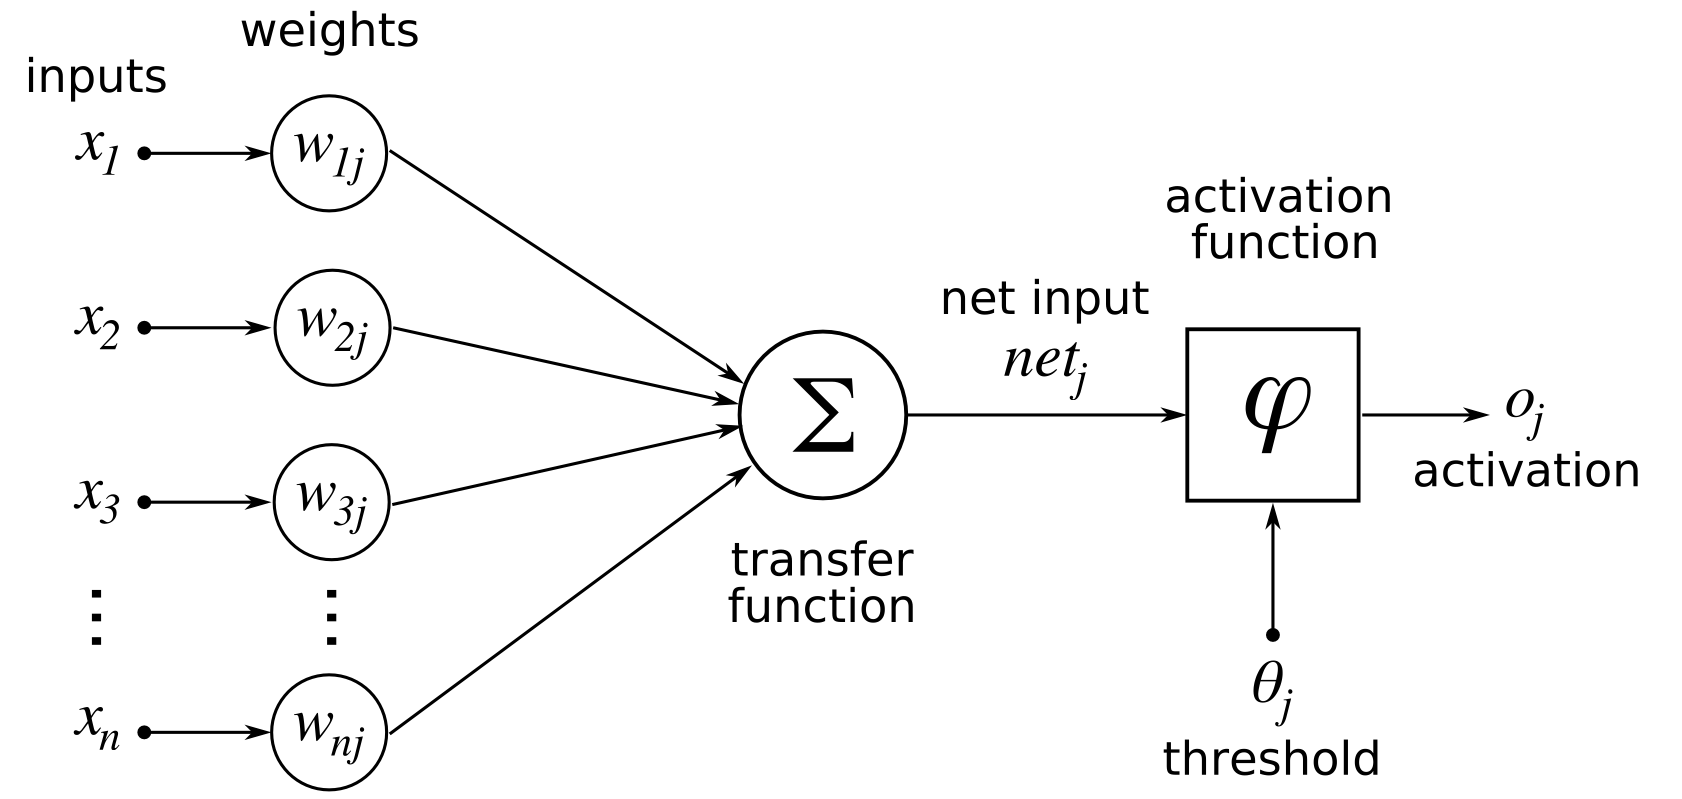
\includegraphics[scale=0.2]{ArtificialNeuronModel_english}
\caption{The Artificial Neuron (Perceptron) \protect\footnotemark}
\label{fig:perceptron}
\end{figure}
\footnotetext{\url{https://en.wikipedia.org/wiki/Talk:Artificial_neuron}}

To learn more powerful models that can perform more complex tasks, the perceptron units are grouped in layers, and these layers are stacked to build deep neural networks (also called multilayer perceptron -- MLP). Traditionally, there are three types of layers; input layers which receive the instances of the data, output layers which produce the results of the network's computations, and hidden layers which lie in between input and output layers and are responsible for computing hidden representations of the previous layers' outputs. The deeper (i.e. latter in the stack) the hidden layer, the more complex representations it is supposed to learn. A network is considered deep when it has two or more hidden layers. In this context, we are more interested in dense layers or fully connected layers, that is layers that have connections between all the neurons.

A deep neural network -- shown in \cref{fig:deep_network} -- is a machine learning (ML) algorithm that uses a hierarchical sequence of $n$ parametric functions to model the input $\mathbf{x}$. Each function $f_i$ ($i \in \{1, 2, \ldots, n\}$)  is modeled as a layer of neurons that apply the perceptron algorithm on the previous layer's output. As a generalization of the perceptron, each layer $l_i$ is parameterized by a weight matrix $\mathbf{W}_i$ applied on the immediate input of $l_i$. Formally, a deep neural network computes the following function:
\[ \hat y = f_n( \mathbf{W}_n, f_{n-1}( \mathbf{W}_{n-1}, \ldots, f_1 (\mathbf{W}_1, \mathbf{x}) ) ) \]

\begin{figure}[ht]
\centering
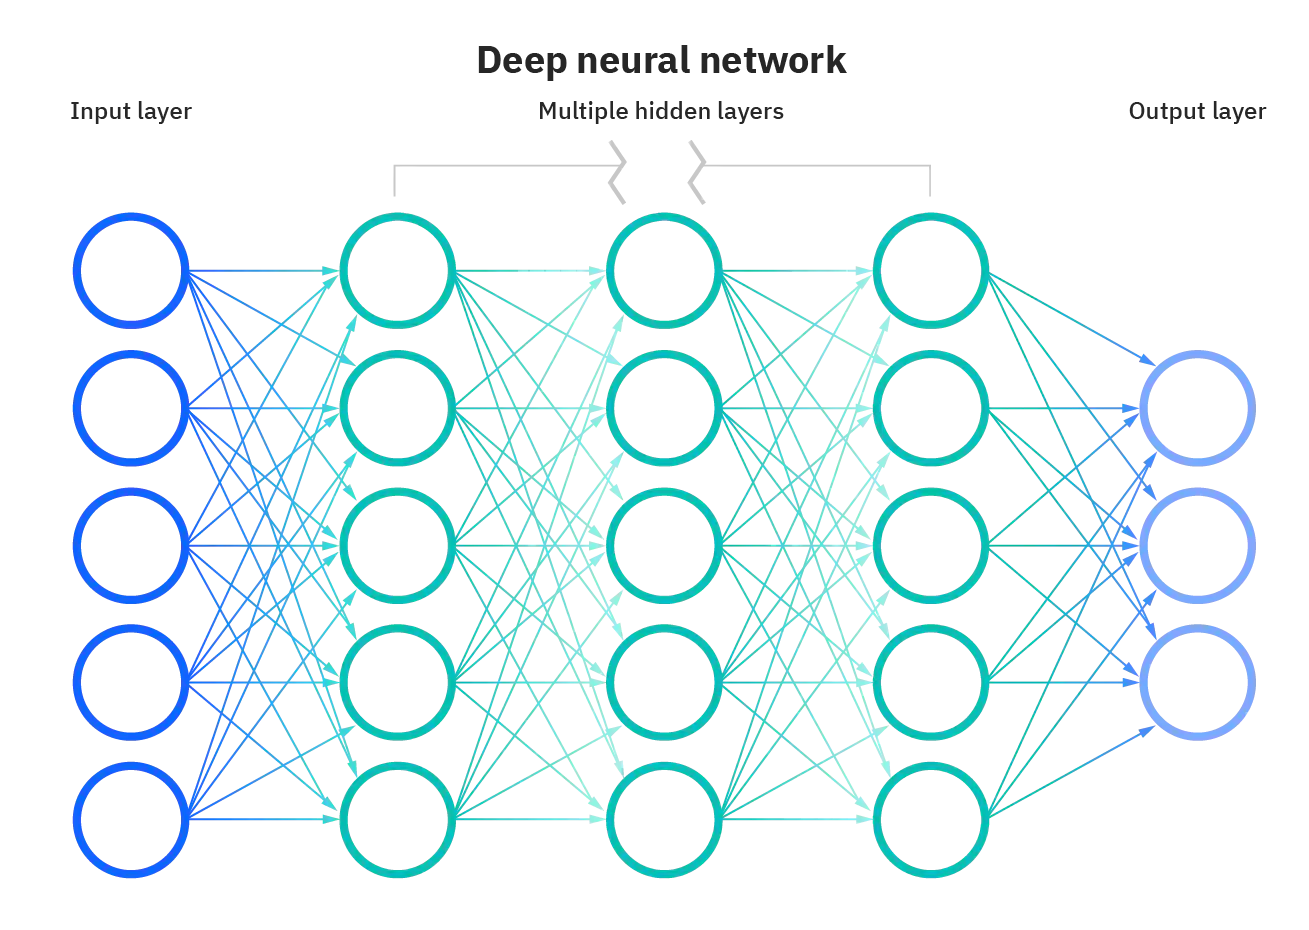
\includegraphics[scale=0.2]{DeepNeuralNetwork}
\caption{Deep Neural Network \protect\footnotemark}
\label{fig:deep_network}
\end{figure}
\footnotetext{\url{https://www.ibm.com/cloud/learn/neural-networks}}

The ability to learn is the key concept of neural networks. During the training phase, the network tries to find the optimal parameters $\mathbf{W}_i, \; i \in \{1, 2, \ldots, n\}$ for solving a given task. Before the training process, the parameters are initialized to some random values which are tuned later according to some error measure. Learning is then carried through an iterative process where we feed the data to the network (called forward pass), analyze the outputs, and repeatedly tune the network for better performance. The outputs are analyzed through a cost function  $J(\hat y, y)$ that measures the error between the prediction $\hat y$ and the true label $y$ for the associated input vector $\mathbf{x}$. The weight tuning procedure is, formally, finding the set of optimal parameters that minimize the cost function $J$. This is done by using the backpropagation algorithm (BP), which computes the gradients of the cost function with respect to the network's parameters ($\nabla_{\mathbf{w}} J$), and then propagates them back from the output layer to the input layer to determine the weight update value according to the formula:
\[ \mathbf{w}^{t+1} \leftarrow  \mathbf{w}^{t} - \eta \ \nabla_{\mathbf{w}} J  \]

where $\eta$ -- the learning rate, defines the amount of weight adjustment. In the evaluation phase, the network's parameters are frozen and the predictions are obtained through a forward pass.

Activation functions are functions that map the input space to a different output space, and they control the information flow between layers in an MLP. These functions have to be continuously differentiable to allow gradients to flow in the backward pass of BP.

According to the universal approximation theorem \citep{csaji2001approximation}, neural networks are universal function approximators. That is, an arbitrary continuous function can be approximated using an MLP with one hidden layer and an arbitrary number of neurons in that layer. For this theorem to hold, the activation functions need also be non-linear, so that the output is non-linearly dependent on the input.

The most commonly used activation functions are \texttt{sigmoid}, \texttt{softmax}, \texttt{tanh} and \texttt{relu} among others.


% =================================================================================================

\section{Word Embeddings}
\label{sec:embeddings}

Deep neural networks deal with numbers and not symbols. In general, an embedding is a representation of a symbol (e.g., word, character, or sentence) in a low-dimensional space of continuous-valued vectors. In natural language, words are not discrete isolated symbols, rather they are correlated with each other. Projecting these continuous-valued vectors into euclidean space visualizes the relationships between words. Depending on the task, we can learn the similarity (distance in Euclidean space) between different word representations.

Word2Vec \citep{mikolov2013distributed} aims to learn a universal embedding matrix $\mathbf{E} \in \mathbb{R}^{V \times d}$ where $V$ is the vocabulary size and $d$ is the dimension of the vector representation. Each row $\mathbf{e}_i$ of $\mathbf{E}$ corresponds to the unique embedding of token $i$ in the vocabulary $V$. This can be learned through one of two methods: continuous bag-of-words (CBOW) or skip-gram. In CBOW, the model predicts the current word from a window of adjacent context words, while skip-gram is the reverse.

Traditional word embeddings suffer from their inability to discriminate different meanings of the same words under different contexts \citep{camacho2018word}. For instance, the word \textit{bank} can refer to two different meanings depending on the context: a financial institution or a sloping land near a body of water. Such words are said to be ambiguous and each meaning is called a word sense.

Sense embeddings attempt to model individual word senses into independent vector representations. This technique mainly relies on fixed sense inventories curated by linguistic experts, such as WordNet \citep{miller1995wordnet}. A sense inventory is a lexical resource (e.g., dictionary) that for each word lists all the possible meanings associated with it \citep{camacho2018word}.

Contextualized embeddings techniques also attempt to solve the problem in an unsupervised way. ELMo \citep{peters2018deep} associates each token with a representation that is a function of the input sequence. These vector representations are obtained from a Bi-LSTM (\cref{sec:birnns}) that is trained with an LM \footnote{A language model is a probability distribution over sequences of words.} objective. ELMo representations are deep, where they are a function of all internal layers of the Bi-LSTM. The higher-level layers capture context-dependent information, while lower-levels capture syntactical information.


% =================================================================================================

\section{Recurrent Neural Networks}
\label{sec:rnns}

Many problems attempted in AI are of sequential and/or temporal nature. Language texts, speech signals, stock prices, and successive video frames are just some examples of real-life applications. Humans normally reason about situations with respect to previous experiences. For example, when reading a language text, each word is thought of in the context of previous words (and maybe future ones). An MLP would be able to output a prediction for every single input, but would not be able to capture the temporal correlation between successive inputs.

To this end, recurrent neural networks were introduced \citep{hochreiter1991untersuchungen}. An RNN differs from a feedforward network by a feedback loop that connects the current input with past inputs to the RNN -- as shown in \cref{fig:rnn_rolled}. Consuming its past outputs as current inputs, the RNN is said to have a memory mechanism where it can take into account past inputs into making a decision.

\begin{figure}[ht]
\centering
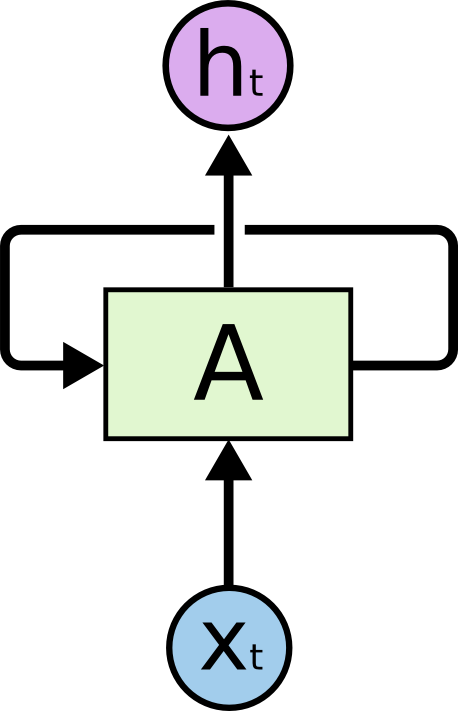
\includegraphics[scale=0.5]{RNN-rolled}
\caption{Recurrent Neural Network \protect\footnotemark}
\label{fig:rnn_rolled}
\end{figure}
\footnotetext{\url{https://colah.github.io/posts/2015-08-Understanding-LSTMs/}}

The sequential information is preserved in the hidden state of the RNN, which spans many time steps as it cascades forward to affect the processing of future inputs. This builds a correlation between temporal events that was impossible to do in MLPs. Since an event or input may depend on a far (in time) predecessor, these correlations are called ``long-term dependencies''. Mathematically this information cascade can be modeled as the recursive relation:
\[ \mathbf{h}_t = f (\mathbf{W}_x \cdot \mathbf{x}_t + \mathbf{W}_h \cdot \mathbf{h}_{t-1}) \]

where $\mathbf{W}_x, \mathbf{W}_h$ are weight matrices and $f$ is an activation function. That is to say; the hidden state at the current time step $\mathbf{h}_t$ is a function of the current input $\mathbf{x}_t$ and the hidden state at the previous time step $\mathbf{h}_{t-1}$.

RNNs are trained through an extension of backpropagation called backpropagation through time (BPTT) \citep{werbos1988generalization}. Time, in this context, is modeled as an ordered series of calculations linking one time step to the next, allowing backpropagation to work.


\subsection{Bidirectional Recurrent Neural Networks}
\label{sec:birnns}

One of the flaws of vanilla RNNs is that it suffers from the limitation of using input information just up to the present time step. In word classification applications that rely heavily on context (e.g., named entity recognition), vanilla RNNs fall short. The limitation restraints the RNN from learning any information about the future context. In fact, an easy solution was proposed \citep{schuster1997bidirectional} by stacking two RNNs, one working in the forward direction while the other works in the backward direction.

A Bidirectional RNN (Bi-RNN) is a composition of two RNNs, where the input sequence is fed normally to the first network and fed in reverse to the second one -- as shown in \cref{fig:bi_rnn}. At any time step $t$, the Bi-RNN would have learned two representations of the input text; $h_{t-1}$ the hidden representation of the past inputs up to input $x_t$, and $h'_{t-1}$ the hidden representation of the future inputs after the input $x_t$.

\begin{figure}[ht]
\centering
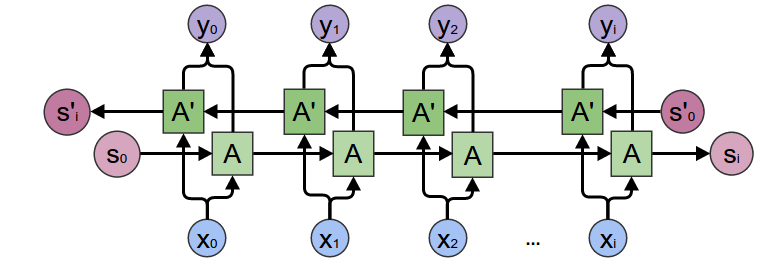
\includegraphics[scale=0.5]{RNN-bidirectional}
\caption{Bidirectional Recurrent Neural Network \protect\footnotemark}
\label{fig:bi_rnn}
\end{figure}
\footnotetext{\url{https://colah.github.io/posts/2015-09-NN-Types-FP/}}

Mathematically, the information propagation is modeled similarly to the RNN:
\[ \mathbf{h}_t = f (\mathbf{W}_x \cdot \mathbf{x}_t + \mathbf{W}_h \cdot \mathbf{h}_{t-1}) \]
\[ \mathbf{h}'_t = f' (\mathbf{W}'_x \cdot \mathbf{x}_t + \mathbf{W}'_h \cdot \mathbf{h}'_{t-1}) \]

Bi-RNNs are trained similarly to RNNs since the two stacked networks are independent of each other. However, applying BP to Bi-RNNs is exceedingly slow due to the very long dependency chain.

\subsection{Long Short-Term Memory Networks}
\label{sec:lstms}

A fundamental problem for vanilla RNNs is vanishing or exploding gradients. As RNNs became deeper to process longer sequences, the successive multiplication of the gradients through the many layers leads to the gradients becoming exceedingly small or large, thus making the learning process unstable. Exploding gradients can be easily handled through clipping or squashing.

Vanishing gradients, however, can cause a network to stop learning by not updating the weights. Long Short-Term Memory (LSTM) networks \citep{hochreiter1997long} were designed specifically to solve this problem. The LSTM unit replaces the standard RNN memory cell to preserve and control the gradient flow during backpropagation.

An LSTM unit as shown in \cref{fig:lstm_cell} consists of a cell and a gating system that controls the information flow through the cell. This control is based on the information's magnitude and importance, through a filtering system that is adjusted through the training process. This filtering system is composed of three gates; forget gate, input gate, and output gate.

\begin{figure}[ht]
\centering
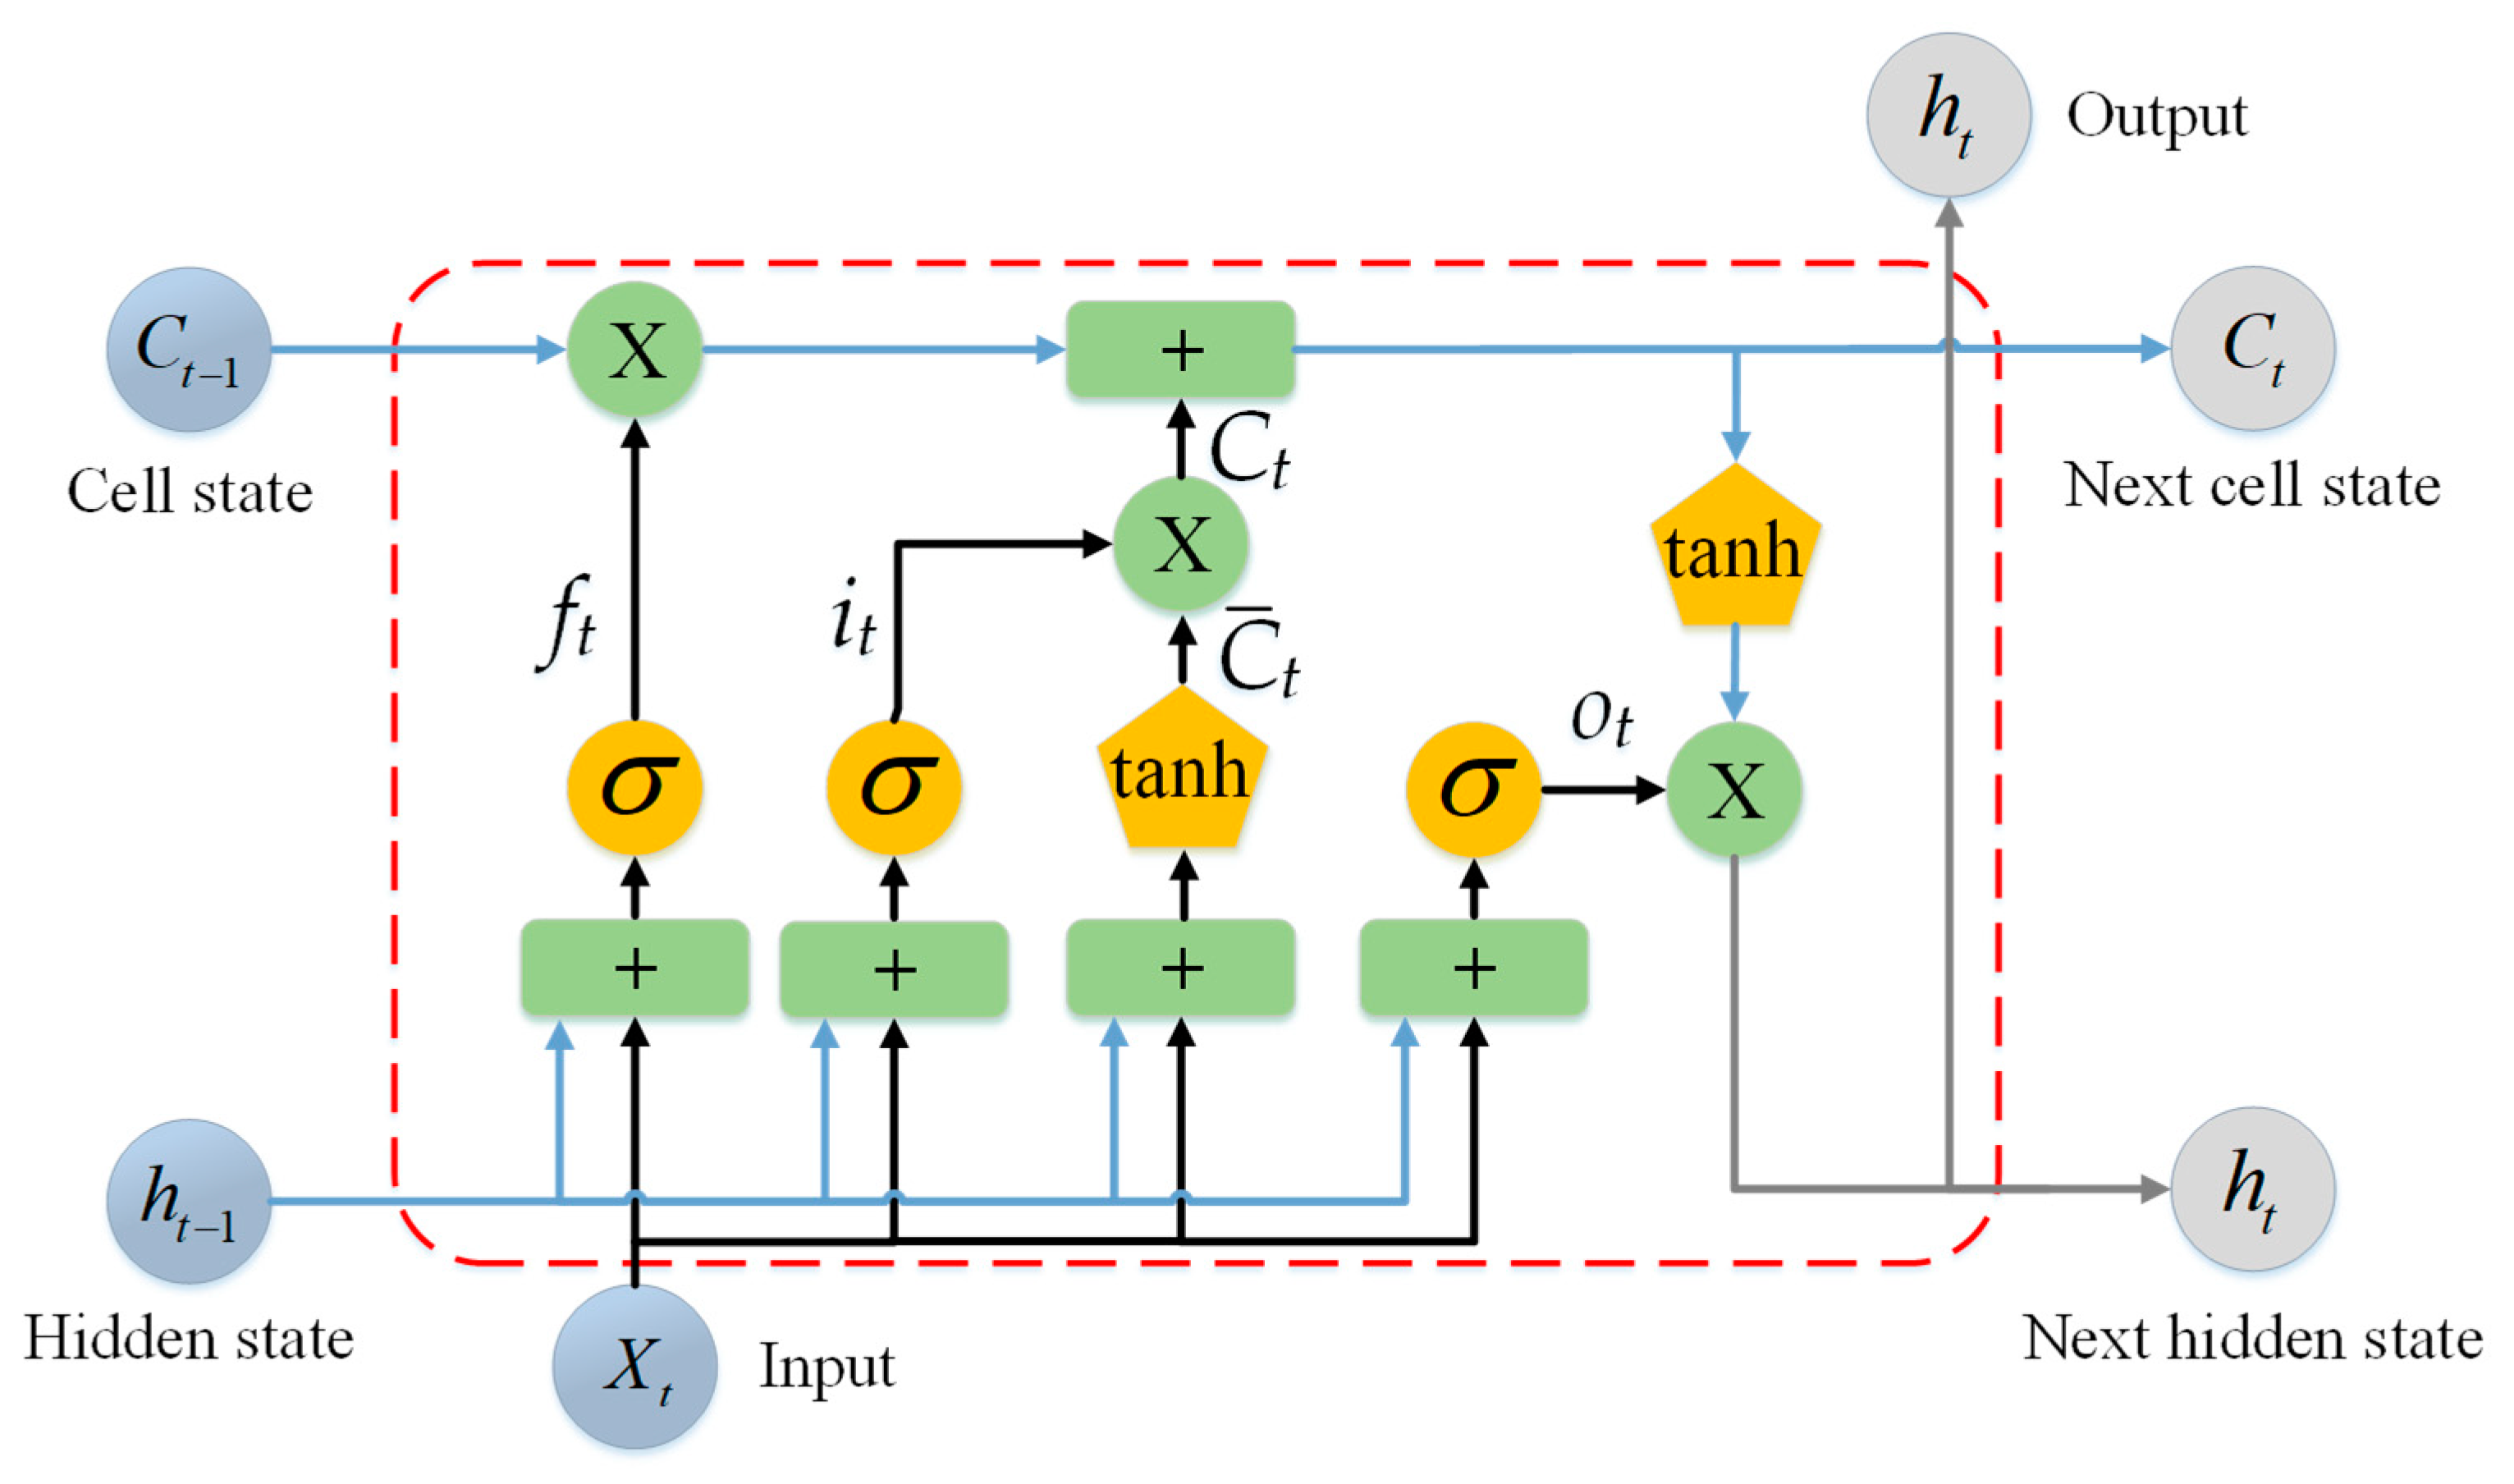
\includegraphics[scale=0.1]{LSTM-cell}
\caption{LSTM Unit \protect\footnotemark}
\label{fig:lstm_cell}
\end{figure}
\footnotetext{\url{https://www.mdpi.com/2079-9292/10/9/1026}}

The core idea behind LSTMs is manipulating the cell state by having the ability to remove, retain or add information to the cell state, regulated by the three gates. Gates learn to optionally let information through. They are composed of a sigmoid layer and a pointwise multiplication operation. The sigmoid output produces a weight [0, 1] of how much information should flow through the gate.

The forget gate decides what information is going to be removed from the cell state. It observes $h_{t-1}$ and $x_t$, and outputs a weight for every value in $C_{t-1}$. This mechanism is useful when the context changes for example. If our subject changes from one sentence to another, we want the LSTM to forget about the old subject and pay attention to the new one. The forget gate learns the following function:
\[ f_t = \sigma (\mathbf{W}_f \cdot [h_{t-1}, x_t] + b_f) \]

In order to register new information, the input gate is used to update the cell state. This is a two step process, first, we decide which values to update. Then, we create a candidate vector $\tilde{C}_t$ that would replace some elements in the cell state.
\[ i_t = \sigma(\mathbf{W}_i \cdot [h_{t-1}, x_t] + b_i) \]
\[ \tilde{C}_t = \tanh ( \mathbf{W}_C \cdot [h_{t-1}, x_t] + b_C ) \]

Next, we perform the cell update. Intuitively, the equation to update the cell state is:
\[ C_t = f_t * C_{t-1} + i_t * \tilde{C}_t \]

Finally, the output gate decides which pieces of the cell state to filter out and which to pass through as the output of the LSTM unit. We squish the cells state with a \texttt{tanh} activation and multiply it by the learned output gate to obtain the new hidden state $h_t$.
\[ o_t = \sigma (\mathbf{W}_o \cdot [h_{t-1}, x_t] + b_o) \]
\[ h_t = o_t * \tanh (C_t) \]

Training an LSTM network means repeatedly adjusting the weights for each gate to learn the optimal behavior to solve a specific task. A popular variant of the LSTM is the Gated Recurrent Unit (GRU). The GRU combines the forget and input gates into a single update gate, and it merges the cell state and the hidden state. The resulting model is much simpler and faster to train without much compromise on  performance.

It is worth noting that while feedforward networks map one input to one output, recurrent structures support a variety of mappings; one-to-many, many-to-one, and many-to-many.


% =================================================================================================

\section{Sequence-to-Sequence Architectures}
\label{sec:seq2seq}

Many applications in NLP are in the form of sequence transformations, that is transforming the input sequence to an output sequence (e.g. machine translation, text summarization, conversational agents), where both sequences can be of arbitrary length. A Sequence-to-Sequence architecture (Seq2Seq) as shown in \cref{fig:seq2seq} consists, mainly, of two networks; an encoder network and a decoder network. In the context of NLP, these networks are typically RNNs or a variant (\cref{sec:rnns}).

The seq2seq model works, first, by scanning the input sequence, token-by-token, with the encoder network. The encoder network is used to ``understand'' the input sequence and learns an associated fixed-size vector representation (context vector) of the whole sequence. The decoder network is initialized with this context vector and proceeds to generate an output sequence, in a token-by-token manner. This decoupling of reading and generation works well in practice on a variety of problems.

Seq2seq models were first introduced \citep{sutskever2014sequence} in the context of machine translation. This new LSTM based model was able to achieve state-of-the-art (SOTA) performance, without the need for any manual feature engineering. The advantage of seq2seq models is the ability to train them end-to-end, assuming the availability of parallel corpora.

\begin{figure}[ht]
\centering
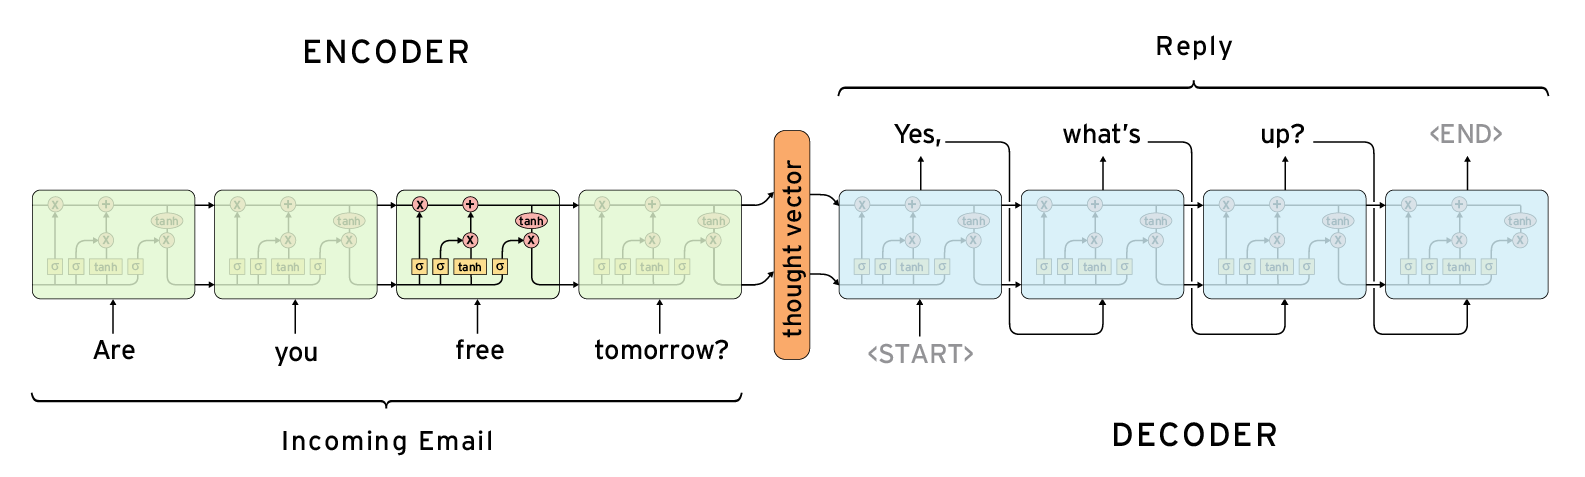
\includegraphics[scale=0.5]{seq2seq}
\caption{Encoder-Decoder Architecture \protect\footnotemark}
\label{fig:seq2seq}
\end{figure}
\footnotetext{\url{https://suriyadeepan.github.io/2016-12-31-practical-seq2seq/}}

The encoder network of the model is of autoencoding property, where it is trained to build a vector representation, of the whole input sequence, that should enable the network to reconstruct the input. In other words, the goal is to learn an efficient encoding that stores the right pieces of information required for reconstruction. Recently, models have been proposed that use the encoder part only of the architecture. Encoders are usually used for language understanding tasks, such as sentence classification or token classification.

The decoder network of the model is of autoregressive property, where it is trained to generate outputs depending on the previous inputs and the hidden state. The decoder defines a probability over the output $\mathbf{y}$ by decomposing the joint probability into conditional probabilities:
\[ p(\mathbf{y}) = \prod_{t=1}^{T_y}  p(y_t \mid \{y_1, \ldots, y_{t-1}\}, \mathbf{c}) \]
with $\mathbf{c}$ being the context vector learned by the encoder.

Similarly, networks with decoder-only components have been in use. Decoders are usually used for language generation tasks, such as text summarization or dialog systems (chatbots).


% =================================================================================================

\section{Attention Mechanism}
\label{sec:attention}

Although seq2seq models work well in practice, the attempt to compress the whole input sequence in a fixed-size context vector is very limiting and sometimes a difficult task. The encoder is very likely to forget some relevant information in longer input sequences. Also, the decoder may need to ``focus'' more on different parts of the input while generating the output at different time steps.

The attention mechanism was first proposed \citep{bahdanau2014neural} to help memorize longer source sentences in neural machine translation. The main concept behind attention is to enable the decoder to have a direct view of the source sequence via the entire sequence of encoder hidden states. These shortcut connections (between the encoder and the decoder) are learnable for each output time step.

Even though the context vector has access to the entire input sequence, its function is now different. Instead of trying to compress the input, it now controls the alignment between the source and target. This alignment is conditioned on: (1) encoder hidden states, (2) decoder hidden states, and (3) alignment weights which represent how well input and output tokens match.

The context vector is computed as a weighted sum of the encoder hidden states:
\[ c_i = \sum_{j=1}^{T_x} \alpha_{ij} h_j \]

The alignment weights $\alpha_{ij}$ are computed by:
\[ \alpha_{ij} = \frac{\exp(e_{ij})}{\sum_{k=1}^{T_x} \exp(e_{ik})}\, , \quad e_{ij} = a(s_{i-1}, h_j) \]
where $e_{ij}$ is parameterized as a feedforward network conditioned on $s_{i-1}$ -- the decoder hidden state and $h_j$ -- the encoder hidden state. This network is trained jointly with other seq2seq components to learn the optimal alignment between target words and source words.

A variety of attention mechanisms have since been studied. We focus on a family of attention mechanisms called self-attention.


\subsection{Self-Attention}
\label{sec:self_attn}

Self-attention \citep{vaswani2017attention} is an attention mechanism that relates different positions of the same sequence to compute a contextual representation of that sequence. The scores of self-attention are computed in parallel which results in an order of magnitude improvement over RNNs, which need to process data sequentially. 

To calculate the self-attention model, we create three distinct representations of the sequence $\mathbf{X}$; $\mathbf{Q} = \mathbf{X} \mathbf{W}_Q$ -- query, $\mathbf{K} = \mathbf{X} \mathbf{W}_K$ -- key, and $\mathbf{V} = \mathbf{X} \mathbf{W}_V$ -- value, with $\mathbf{W}_Q, \mathbf{W}_K, \mathbf{W}_V$ learnable weight matrices. This query-key-value concept is borrowed from information retrieval systems. When you search for a \textit{query}, the search engine will map the query against a set of \textit{keys} associated with possible results. Then an algorithm will return the best-matching results (\textit{values}).

This process in information retrieval literature is called content-based lookup \citep{mitra2000information}, hence the name \textit{content-based} self-attention. In the self-attention mechanism, this idea of retrieving an object is relaxed. We define a degree of similarity between our representations to be able to weigh our query. Instead of choosing where to look depending on the position in the sequence, we can attend to the content we need itself. That is why we need to separate keys from values; the keys are used to calculate the attention weights while the values define the information we \textit{retrieve}.

We can now define the self-attention mechanism mathematically:
\[ \text{Self-Attention}(\mathbf{Q}, \mathbf{K}, \mathbf{V}) = \text{softmax} \Big(\frac{\mathbf{Q} \mathbf{K}^T}{\sqrt{d_k}}\Big) \mathbf{V} \]
where we notice the similarity measure using a scaled dot-product. The scaling is to prevent the problem of exploding gradients. The \texttt{softmax} activation is used to get the final attention weights as a probability distribution.


\subsection{Multi-Head Self-Attention}
\label{sec:multihead_attn}

Multi-Head Self-Attention \citep{vaswani2017attention} can be thought of, simply, as an ensemble of independent self-attention mechanisms running also in parallel. In this context, the output of a single self-attention model is called a ``head'', the outputs of different heads are concatenated and linearly transformed into the expected dimension (see \cref{fig:multi_head_attn}). This composition of heads allows the model to jointly learn different representations of the input which improves the final attention-based representation.
\[ \text{Multi-Head} (\mathbf{Q}, \mathbf{K}, \mathbf{V}) = [\text{head}_1; \ldots; \text{head}_n] \mathbf{W}_O \]
where each head is the output of the scaled dot-product attention (\cref{sec:self_attn}).

\begin{figure}[ht]
\centering
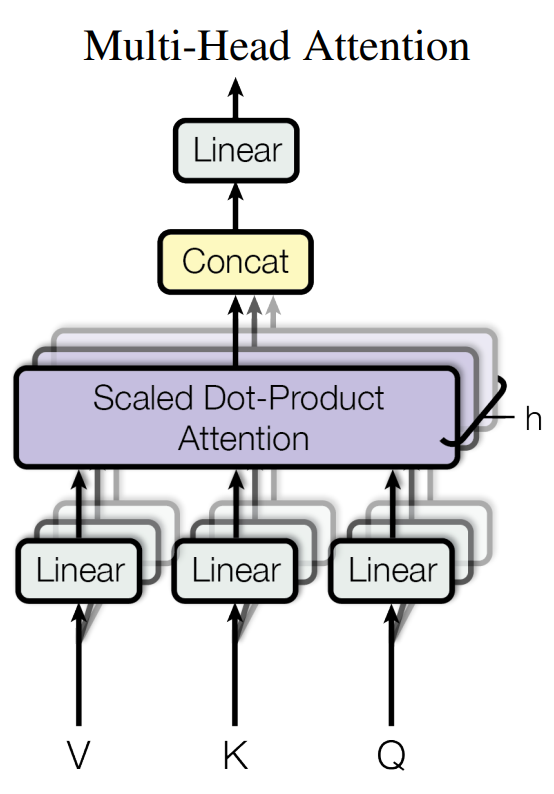
\includegraphics[scale=0.3]{multi_head_attn}
\caption{Multi-Head Self-Attention \protect\footnotemark}
\label{fig:multi_head_attn}
\end{figure}
\footnotetext{Attention is all you need. \citep{vaswani2017attention}}


% =================================================================================================

\section{Transformers}
\label{sec:transformers}

Recurrent architectures process input data sequentially to build a vector representation that is used in downstream tasks. Several models have been proposed to improve this limitation and have sequential data processed in parallel. ByteNet \citep{kalchbrenner2016neural} and ConvS2S \citep{gehring2017convolutional} use convolutional neural networks (CNNs) as basic building block to compute hidden representations in parallel for input and output positions. In these models, the number of calculations required to relate two arbitrary input and output positions grows in the distance between positions, linearly for ConvS2S and logarithmically for ByteNet. This makes it more expensive to learn representations for longer sequences.

The Transformer architecture was introduced \citep{vaswani2017attention} to solve this problem. Transformers are entirely built on the multi-head self-attention mechanism, without any recurrent units. The number of required calculations required to relate two arbitrary positions is now constant.

The Transformer is an encoder-decoder architecture -- shown in \cref{fig:transformer} -- based on multi-head self-attention modules and normalization layers with residual skip connections.

An encoder block consists of: (1) multi-head self-attention layers (discussed in \cref{sec:multihead_attn}), (2) feedforward layers applied on the attention layer output to project it in a higher-dimensional space, (3) residual skip connections which are shortcut connections to add the input of the sub-layer to its output; this was found to improve gradient flow while adding more layers, and finally, (4) layer normalization \citep{ba2016layer} which independently normalizes the vector representation for each token -- this improves convergence stability.

A decoder block is similar to an encoder block with exceptions. The first multi-head attention is modified to mask the latter positions to prevent the decoder from attending to subsequent positions during predicting the current token. The second multi-head attention takes input from both the previous sub-layer and the encoder.

\begin{figure}[ht]
\centering
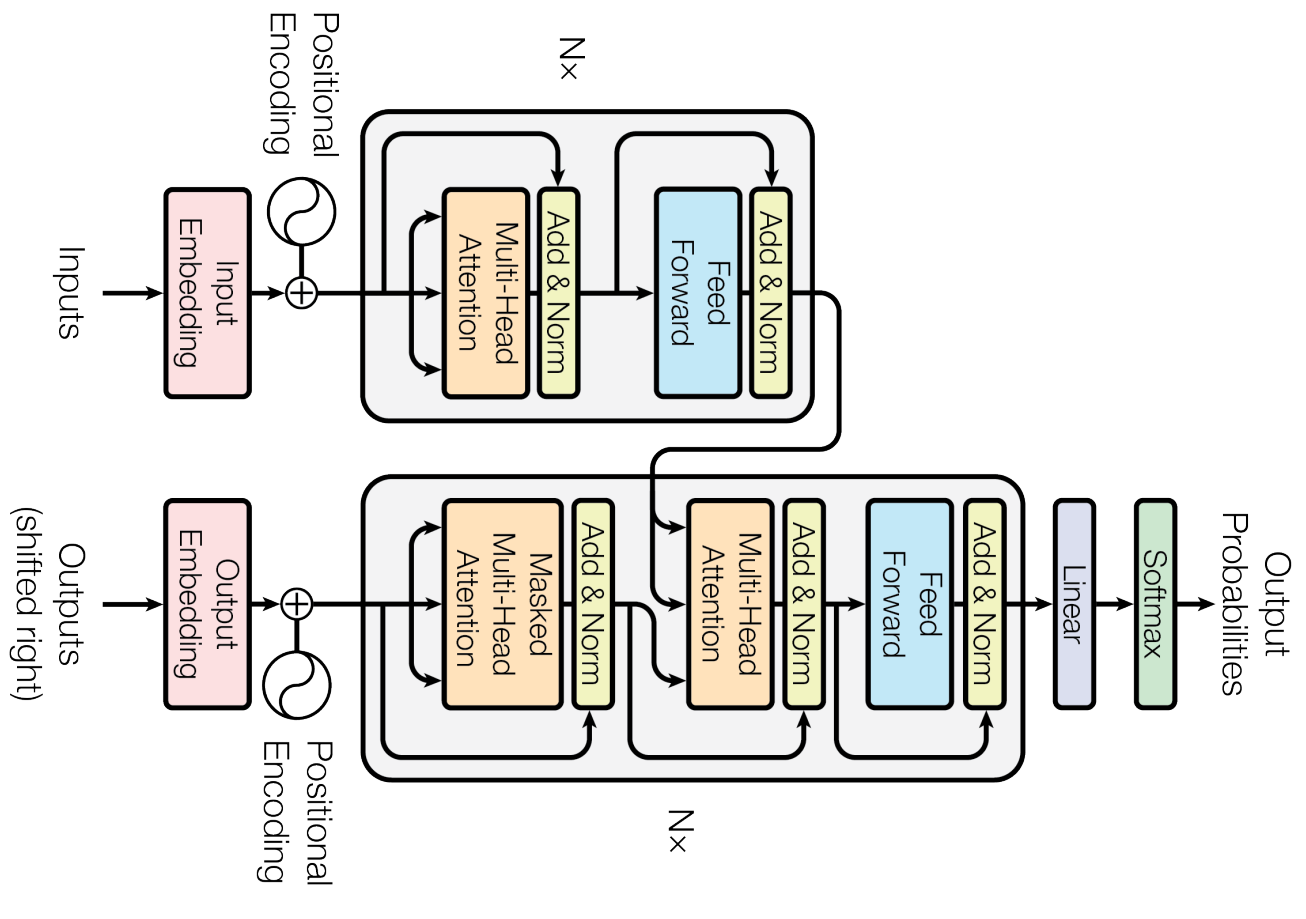
\includegraphics[scale=0.3, angle=90]{transformer}
\caption{Full Architecture of the Transformer. Encoder (left) and Decoder (right). \protect\footnotemark}
\label{fig:transformer}
\end{figure}
\footnotetext{Attention is all you need. \citep{vaswani2017attention}}

\subsection{Positional Embeddings}
\label{sec:pos_embeddings}

All word embedding techniques (\cref{sec:embeddings}) incorporate information about the token's position in some way -- a context window, a recurrence, or a convolution. However, in Transformers we completely remove the sequential processing mechanism of the RNN in favor of the parallelism of self-attention. In turn, this led to the loss of positional information for input tokens.

The authors of the original Transformer paper \citep{vaswani2017attention} introduced a function $f \colon \mathbb{N} \mapsto \mathbb{R}^d$ to compute the positional encoding $p_t$ for a token at position $t$ as follows:
\[
p_t^{(i)} = f(t) ^ {(i)} = \begin{cases}
	\sin(\omega_k \cdot t), & \text{ if } i = 2k \\
	\cos(\omega_k \cdot t), & \text{ if } i = 2k + 1\\
\end{cases}
\]
where $\omega_k = \dfrac{1}{10000^{2k/d}}$ and $i$ is the dimension. This output vector $p_t$ is then added to the input embeddings -- where they have the same size.

This type of embeddings was chosen since: (1) it is unique and deterministic for each token, (2) allows the model to generalize to longer sequences than those encountered in training, and (3) allows the model to attend by relative positions efficiently.

Finally, thanks to the use of residual skip connections through the Transformer blocks, the positional information is efficiently propagated to higher-level layers where more complex interactions are handled.


\subsection{Pretrained Transformer Models}
\label{sec:pretrained_models}

The ability to train models quickly through enhanced hardware capabilities combined with improved learning algorithms has led to a paradigm shift in deep learning. In NLP, this shift came with the rise of transformers which could be trained faster, by order of magnitudes, than recurrent architectures and on longer sequences with better results.

Transfer Learning is a method of reusing the information (weights) learned by one trained model, on some task, in another model that is required to perform a different but related, task \citep{Goodfellow-et-al-2016}. This is done by using \textit{pretrained} models in some way. One can either continue training those learned weights on the required task (fine-tuning) or simply freeze the weights and train only the output layer.

Transfer learning opened the window for accessible state-of-the-art models to be used in all scenarios without the difficult requirements of obtaining such models.

\subsubsection{BERT}
\label{sec:bert_intro}

One of the most famous pretrained transformer models is BERT which was developed by Google. BERT \citep{devlin2018bert} -- or Bidirectional Encoder Representations from Transformers -- outperformed other NLP models when it was released in many language-related tasks. It builds on top many clever ideas that were proposed by several researchers, like semi-supervised sequence learning \citep{dai2015semi}, ELMo \citep{peters2018deep}, ULMFiT \citep{howard2018universal}, and the Transformer \citep{vaswani2017attention} among others.

BERT uses encoder blocks from the vanilla transformer and is most suitable for language understanding tasks (e.g., sequence classification, next token prediction). The first innovative addition in BERT is that it uses a bidirectional self-attention mechanism in contrast to left-to-right self-attention used in the vanilla transformer. This idea leads to an improved contextual representation for tokens. However, it also creates a problem where each word would be able to attend to itself in a multi-layered context, thus leading to corrupted training.

To solve this problem, the authors propose to randomly mask some of the input tokens and have the model learn how to reconstruct these tokens based on the context. This task is called Masked Language Modeling (MLM). The mask's value can be a generic value or sometimes a word is replaced with another to improve fine-tuning on downstream tasks.

Another pretraining task used is Next Sentence Prediction (NSP). Many downstream tasks require the understanding of the relationship between two sentences (e.g., Question Answering, Natural Language Inference). This task is cast to a binary classification task where BERT simply decides whether the latter sentence follows the first.

After pretraining BERT on the two previously mentioned tasks, it can be fine-tuned to solve a variety of language understanding problems. One other way to use BERT is as a feature extractor, where BERT is used to produce contextual word embeddings which are then fed to any model of choice on some related task.

\subsubsection{BART}
\label{sec:bart_intro}

BERT-like models perform well where the prediction at position $i$ is allowed to use information from later positions. This is, however, not practical in text generation tasks, where the prediction for position $i$ can depend only on previous positions. On the other hand, autoregressive models, such as GPT \citep{radford2018improving}, are pretrained to predict the next word while masking future positions making it more suitable for generation tasks. It follows that GPT-like models are unable to generalize well on downstream tasks where the whole input contributes information for the output.

BART \citep{lewis2019bart} combines the best of both approaches. It utilizes the full transformer architecture, with a BERT bidirectional encoder and a GPT autoregressive decoder, along with a variety of pretraining tasks. BART is pretrained on (1) token masking similar to BERT, (2) token deletion, where random tokens are deleted and the model must predict their correct positions, (3) text infilling, where a span of text (sequence of tokens) is masked by a single mask and the model must predict how many tokens were masked, (4) sentence permutation, where sentences of a document are shuffled in random order, and finally, (5) document rotation, where a document is rotated to start from a given token and the model is asked to predict the correct starting token.

BART performs best when fine-tuned on text generation tasks, but also works well for language comprehension tasks.



\chapter{Related Work}
\label{ch:related_work}

% https://mark-riedl.medium.com/an-introduction-to-ai-story-generation-7f99a450f615

% grammar based approaches
In cognitive science, story grammars view stories as scripts -- structures that describe a sequence of events in a particular context \citep{schank2013scripts}. This comes from the fact that in most situations, events usually occur in stereotypical patterns. These patterns are used as schemas or grammars to guide story generation. Structured story generation is to automatically generate stories by dividing the stories into slots following a given schema. Slots are then filled by selecting similar plots from previously annotated stories \citep{alhussain2021automatic}.

Propp's model was one of the earliest to formalize stories into structural models \citep{propp1968morphology}. Propp studied hundreds of Russian folktales and concluded that they follow a similar global structure. He extracted 31 functions (character actions) of which a subset is sure to drive any given story.

Inspired by Propp's analysis, JE Grimes pioneered the field of automated story generation in the early 1960s. Grimes used the Monte Carlo approach to randomly sample a subset of Propp's functions and order them based on a set of intelligent grammar rules to build a story as seen in \cref{tab:grimes-story-sample} \citep{ryan2017grimes}. Back then story generators were non-learning rule-based systems that focused on the quality of a certain aspect (e.g., syntax or plot...). In the 1970s and 1980s, several researchers published story grammars which are necessary for story understanding and generation \citep{rumelhart1975notes, thorndyke1977cognitive, wilensky1983story}.

\begin{table}[h]
\centering
\begin{tabular}{p{0.9\linewidth}}
\hline
\uppercase{A lion has been in trouble for a long time. A dog steals something that belongs to the lion. The hero, lion, kills the villain, dog, without a fight. The hero, lion, thus is able to get his possession back.} \\ 
\hline
\end{tabular}
\caption{One of the first computer-generated stories by JE Grimes}
\label{tab:grimes-story-sample}
\end{table}

Nevertheless, grammar-based approaches focus only on the syntax of the story rather than the semantics. Logical relationships between story events and character goals are ignored which affects the story coherence and believability \citep{alhussain2021automatic}. Also, structural models are restricted to a certain domain and cannot modify their knowledge rules to generate different stories.

% planning based approaches
The realization that story generation is a \textit{creativity} problem begged the usage of more intelligent techniques. Story planners assume that narrative generation is a goal-driven process and apply a symbolic planner to generate a story. In this context, a story is viewed as a chain of causally related events (story points) that satisfy an end goal. Such systems are restricted to solve a theme and can easily delimit the path followed to generate a story \citep{herrera2020automatic}.

The first widely-known system to use a planner is TALE-SPIN \citep{meehan1977tale}. This system generates different characters with their respective goals and proceeds to find a resolution of these goals using an inference engine based on common sense reasoning theories. TALE-SPIN showed a substantial improvement over Grimes' fairy tales system, thanks to the ``reasoning'' capability provided by the inference engine.

Thanks to Meehan's work in TALE-SPIN and the modern formalization of symbolic planning in predicate logic, many works that use planners for story generation in different approaches came to be \citep{dehn1981story, lebowitz1984creating, lebowitz1985story, cavazza2002character, porteous2009controlling, riedl2010narrative}. However, many stories generated using planners had an inherent problem; each step depends only on the current state of the story and not past states.

% case/analogy based approaches
Drawing from cognitive theories, computational analogy identifies similarities and transfers knowledge from a source domain to a target domain \citep{zhu2013shall}. This approach is applied in story generation systems by searching the knowledge bases for a story world state similar to the current story world, then the next state in the knowledge base would be the new state for the generated story. The similarity measure would depend, in this context, on the generation system.

MINSTREL \citep{turner1993minstrel} is one the earliest analogy-based generators. It is driven by character and author goals where case-based reasoning is used to resolve the goals. The system stores the cases in its memory and indexes them by important features such as locations and actions to group related cases. The system then adapts these cases/scenes through a model of computational creativity to ensure novelty. Similarly, MEXICA \citep{perez2001mexica} uses a method of engagement and reflection, to use already known narratives and generate a new story that maintains coherence, novelty, and an increasing tension throughout the story.

% heuristic search approaches
To increase the variety of generated stories, the stories search domain needs to be expanded. However, as the search space increases, it becomes more difficult for planners to find a solution. Heuristic search techniques were used to find a story in a story search space. HEFTI \citep{ong2004genetic} and PlotGA \citep{mcintyre2010plot} use Genetic Algorithms to search for plot points and then generate a narrative. \citep{cavazza2009emotional} use real-time A* for story generation in an interactive setting.

% transition to ML
With the recent boom in learning algorithms and hardware capabilities, the focus started to shift from symbolic rule-based systems to learnable generation techniques. Machine Learning (ML) methods can be used for knowledge acquisition, in contrast to non-learning systems which need prior encoding of schemas and scenarios. Most ML systems, in the context of story generation, attempt to model, probabilistically, the process of writing a story in some way. After a probability distribution is learned, the model is then able to sample from this learned distribution to generate a new story.

Different works classify recent story generation systems according to different criteria. \citep{hou2019survey} use the constraints applied to the generation process to separate systems. \citep{herrera2020automatic} survey different systems according to the type of guideline used to generate the story. \citep{alhussain2021automatic} differentiate between required tasks in the domain of story generation; filling the gaps, ending completion, and from-scratch generation.

We use Hou's system of classification which organizes story generators into theme-oriented models, storyline-oriented models, and human-machine interaction-oriented models \citep{hou2019survey}. Theme-Oriented models are characterized by a consistent theme throughout the whole generation process. Storyline-Oriented models are constrained by complete story plots to guide the generation. Story plots are forms of abstract descriptions of the development of the storyline, and can also be in the form of a given story that needs a suitable ending. Finally, Human-Machine Interaction-Oriented models are dynamic with user input guiding the generation process.


% =================================================================================================

\section{Theme-Oriented Models}
\label{sec:theme_models}

Theme-oriented models refer to models in which the user constraint is static and gives a high-level description of the story's topic/theme. This type of models has the highest degree of flexibility and weakest constraints on the generation process which results in a difficulty of generating consistent, coherent, and vivid stories \citep{hou2019survey}. In this section, we review some of the methods that follow this paradigm.

\citep{choi2016recurrent} use two RNN encoder-decoder LMs to generate a story. The first network maps an input sentence to a vector representation, while the second network decodes this representation to generate the next sentence in the story. \citep{harrison2017toward} modeled the chain of story events as a Markov Chain and used an RNN to guide a Markov Chain Monte Carlo (MCMC) sampler to generate new stories. RNN-based LMs proved their ability to generate grammatically correct sentences, however, generated stories lacked overall coherence.

\citep{martin2018event} adopted the idea of hierarchically generating the story to improve long-term dependency and global coherence. Martin separated the task into two phases; first generate a sequence of events that outlines the progression of the story, then generate a narrative describing the relationships between the events. An event is a 4-tuple $\langle s, v, o, m \rangle$, where $v$ is a verb, with $s, o$ its subject and object respectively, and $m$ is a wildcard which represents a dependency of some kind. To generate the sequence of events, an encoder-decoder network is used with a greedy decoding mechanism. To reconstruct human-readable sentences from the intermediate sequence of events, another encoder-decoder network is used with a beam search decoder to find optimal sentences. 

\citep{xu2018skeleton} draw inspiration from classical schema-based methods and generate a skeleton -- the most critical phrases that reflect the semantic connections between sentences. The skeleton is then further expanded into complete sentences. LSTM-based encoder-decoder networks (with attention decoders) are used for both phases; generating the skeleton from the input, and expanding the skeleton into a fluent story. However, unlike classical methods, skeleton extraction is trained using a reinforcement learning (RL) method to preserve only key information necessary to create a story. The skeleton model show improved coherence and story fluency.

Similarly, \citep{fan2018hierarchical} use a two-step process to generate stories. First, they generate a premise describing the topic of the story then they condition the story generation on this premise. To generate the conditioning prompt, they build on top of the ConvS2S \citep{gehring2017convolutional} LM with a novel gated multi-scale self-attention mechanism to attend to different positions and be able to make better fine-grained selections. Next, to improve the dependency on the conditioning prompt, they use a fusion model -- where a seq2seq network has access to the weights of a pretrained seq2seq network. The goal is for the second network to improve where the first network failed to learn.

\citep{yao2019plan} propose to dynamically generate the story plan adopting experiences from many human writers. Instead of generating the whole plan first then moving on to the story, they generate the plot point and then the corresponding sentence in the story -- thus interleaving the plan and story generation one step at a time.

\citep{yu2020draft} use a modified conditional variational autoencoder (CVAE) in a multi-pass editing scheme to generate a story. The architecture uses a GRU-based encoder with a hierarchical decoder consisting of a global-level decoder responsible for guiding local-level decoders into generating story sentences. They use two CVAEs; the first generates a draft of the story based on the title, then the second consumes both the title and the generated draft to produce the final story. This scheme allows the second CVAE to focus on overall semantic consistency and coherence.

Many other works adopt this hierarchical generation framework \citep{ammanabrolu2019guided, fan2019strategies, zhai2019hybrid, ammanabrolu2020story}. The reason for the wide adoption of this framework is the ability to model the relationship between plot points at a higher level than words and maintain long-term dependencies yielding improved results over standard seq2seq models in terms of global coherence and semantic consistency.

%Since the introduction, the inherent architecture could already provide many of the benefits of using a hierarchical generation approach. That motivated researchers to another formulation of the approach. Instead of generating an abstract representation of the story, they would instead feed this abstract representation as supplementary input to 

The recent success of Transformer models motivated researchers to pursue more complex enhancements to improve the generation process.

\citep{brahman2020modeling} use COMET -- a knowledge base -- to identify the emotional reaction of the main character in each sentence, and then use this ``emotional arc'' to guide the generation. To correctly classify an emotion, they use a pretrained BERT model then finetune it on an emotion identification dataset then further finetune it on an emotion annotated (using COMET) story dataset. Next, they use this classifier loss to optimize the model (GPT-2) to continually align to the emotional arc using a reinforcement learning policy.

\citep{kong2021stylized} use a similar approach where they use stylistic keywords as a higher-level representation for the story. They first learn the probability distribution for the stylistic keywords through an encoder and then use this distribution directly to condition the decoder while generation. The types of styles they consider are emotion-driven and event-driven styles. To extract emotion labels they make use of a lexical tool (NRCLex) and for the event labels, they use NLTK to extract non-common verbs. Finally, to guide the model during generation, they explicitly add a token that signifies the type of style the story should follow.

% maybe move this to another models section
\citep{yu2021sentence} aim to improve the diversity of output text by permuting the sentence order. Their method, PermGen, maximizes the expected log-likelihood of output paragraph distributions with respect to all possible sentence orders. To do so, they use three modules; (1) hierarchical positional embedding, which keeps track of the token's position in the sentence and in the paragraph, (2) sentence-permuted learning, which maximizes the log-likelihood of generating every possible paragraph permutation, and (3) sentence based decoding, which generates the sentences out of order then proceeds to order them according to their rank with log-probability.

\citep{guan2021long} propose two additional pretraining tasks in addition to the language modeling task. The first task is a sentence similarity task where the model learns sentence-level representations to minimize a similarity score using SentenceBERT as a reference. The second task is a sentence ordering task where the model learns discourse-level representation to correctly determine whether two sentences are in order. Coupled with negative sampling, the goal for these extra tasks is to allow the model to effectively capture the high-level semantics and discourse structures in the context.


% =================================================================================================

\section{Storyline-Oriented Models}
\label{sec:storyline_models}

Storyline-oriented models are still characterized by a static user constraint, but in this case, the constraint directly describes plot points which are then used to generate the story. Conceptually, this type of models resembles the second part/phase of theme-oriented models (\cref{sec:theme_models}) where the input is a high-level representation of the plot points and the semantic connections between them.

\citep{huang2016visual} introduced the first dataset for visual storytelling (VIST). They present sets of pictures in sequences coupled with text captions that describe the pictures.

\citep{wang2018no} use an adversarial reward learning framework on VIST to learn an implicit reward function from human experience, and then use this learned function to optimize the generation policy. In their architecture they make use of two models; a policy model that takes an image sequence and takes a sequence of actions (choosing words for the story), and a reward model that computes partial fine-grained rewards for each sentence representation along with the visual features learned from the input image.

\citep{kim2018glac} propose an attention-based approach to encode information between adjacent pictures in VIST. They use a global-local attention mechanism where the global attention focuses on overall semantic correlations while local attentions focus on extracting information from images to generate the story. To output sampled sentences, they use a custom decoding scheme where the probability of sampling a new word is inversely related to its frequency. This prevents repetitive text and insures diversity of generated stories.

Another method to encode storylines is in the form of some intermediate semantic representation. This representation can be a set of abstract sentences or event representations. The need to encode in some abstract representation arises from the fact that stories in their textual form contain many insignificant details and add extra overhead for the learning process. 

\citep{martin2018event} use a 4-tuple to represent an event (discussed in \cref{sec:theme_models}). \citep{mostafazadeh2016caters} make use of a novel annotation framework to simultaneously capture temporal and causal relations between events. \citep{jain2017story} use a set of independent event descriptions to generate coherent stories. \citep{yao2019plan} create a story abstraction by extracting each sentence's most important word.

We add the task of predicting/generating an ending for a story in this section since it requires an understanding of the storyline up to that point. \citep{zhao2018plots} use RL to generate story endings that have high semantic relevance with story plots by applying a copy and coverage mechanism. \citep{hu2017happens} uses a context-aware LSTM to capture the temporal order of past sub-events and generate a prediction of a future sub-event. \citep{guan2019story} argue that generating a rational ending for a story is an indicator of story comprehension since it requires understanding key storyline points and inherent commonsense knowledge.


% =================================================================================================

\section{Human-Machine Interaction-Oriented Models}
\label{sec:interaction_models}

This class of models deals with a dynamic user constraint. The input constraints vary with human interaction and the problem is cast more as an interaction problem rather than an algorithmic one.

\citep{clark2018creative} studied a machine-in-the-loop story generation framework where an LM suggests new sentences to stimulate ideas for the writer. They conclude that participants appreciated creative and diverse suggestions more than random less meaningful ones. \citep{goldfarb2019plan} use different varieties of interaction to improve human engagement. In their system, writers can outline the plot of the story, control the diversity of generated plots and story sentences, edit and modify previously generated content. They show improved user satisfaction with creative and relevant generated content.


% =================================================================================================

\section{Other Models}
\label{sec:other_rel_models}

This section is dedicated to works that are not directly related to automated story generation but contributed to the development of this work.

As discussed previously, the idea of cycle framework was used before in the context of machine-generated language translation by \citep{he2016dual}. They cast the problem as a two-agents game. The first agent (model) translates the message from language A to B and sends the translated message to the second agent. The second agent evaluates the readability of the received message (\textit{not} translation correctness) with respect to language B, translates it back to language A and retransmits it back to the first agent. The first agent then evaluates the reconstruction quality and signals the second agent for feedback. The game is then started the other way around until both models converge. They use RL policy gradient methods to optimize models on the readability of the intermediate sentence and the quality of the reconstructed sentence. Since they use RL for optimization, the training procedure is unstable, the models need pretraining to be able to converge, and the training process needs a big amount of time.

\citep{baziotis2019seq} propose a text compression mechanism using an autoencoder architecture that uses differentiable approximations for text sampling which can use gradient-based optimization leading to better performance over seq2seq models. The compressor is a seq2seq with attention that adaptively determines the length of the compressed sequence. Then they use the Gumbel-softmax reparameterization trick with a straight-through estimator to sample words from the compressor's output distribution. In contrast to argmax sampling, using this sampling method allows for the backpropagation of gradients allowing a gradient-based optimization. The reconstructor is similarly a seq2seq that reconstructs the input again. However, to make the models converge they make use of multiple losses: (1) reconstruction loss, (2) prior loss, which is an LM loss that measures the readability of the compressed text, and (3) a topic loss, which is a TF-IDF based cosine similarity loss that forces the compressed text to draw words from the same distribution as the original text.


% =================================================================================================

\section{Position Of Our Framework}
\label{sec:analysis_prev_work}

The majority of the hierarchical generation methods presented in (\cref{sec:theme_models}) are either recurrent or convolutional-based models which are generally outperformed by the recently introduced Transformers. Moreover, authors of these works still report tendencies to repeated text generation, inconsistencies, incoherency, inability to adhere to the theme, produce shorter stories, copy from input prompt, and focus on and generate more frequent words.

Storyline models (\cref{sec:storyline_models}) adhere too much to the inputs resulting in less generalized and original stories. They are also highly dependent on the input when it comes to generating a coherent and logically consistent story. Additionally, they exhibit some of the problems of theme-oriented models.

Observing the Transformer-based approaches reviewed previously, we see that these methods use complex feature engineering that requires a considerable amount of extra computing power and/or training time. Instead, we propose a much simpler method that provides better results and is easily extendable.

The dual learning algorithm \citep{he2016dual} uses an RL optimization procedure which is inefficient -- since it required a long time to train the models -- and unstable -- where pretraining was required to initialize the models. In contrast, we use a gradient-based optimization algorithm, that proves to be more efficient when training bigger models.

The text compression mechanism \citep{baziotis2019seq} although efficient but still report instability -- where the topic loss is a key factor for convergence. The model also tends to copy words from the original text to the compressed text. Additionally, they report that the model weakly recovers from early errors that have cascading effects.



\chapter{Cycle-consistency Framework}
\label{ch:main_idea}


\graphicspath{ {./body/media/} }


In this Chapter, we detail our approach to automated storytelling. First, we provide a formalization of the problem (\cref{sec:formulation}). Then, we proceed to explain our baseline architecture (\cref{sec:baseline_arch}). Finally, we explain how we build on top of the baseline to get the cycle architecture and some possible extensions (\cref{sec:cycle_arch}).


\section{Problem Formulation}
\label{sec:formulation}

Previously the task of story generation has been mostly viewed as a translation task, where a model is given as input a summary/topic and is required to produce a story. A simple schema is shown in Figure \ref{fig:classical_problem_formulation}. More formally, given a conditional sequence $\mathbf{x} = (x_1, x_2, \ldots, x_{|\mathbf{x}|})$, that indicates a title, a topic or a short summary, the model is required to translate it into a sequence $\mathbf{y} = (y_1, y_2, \ldots, y_{|\mathbf{y}|})$ indicating a story that follows some constraints.

\begin{figure}[ht]
\centering
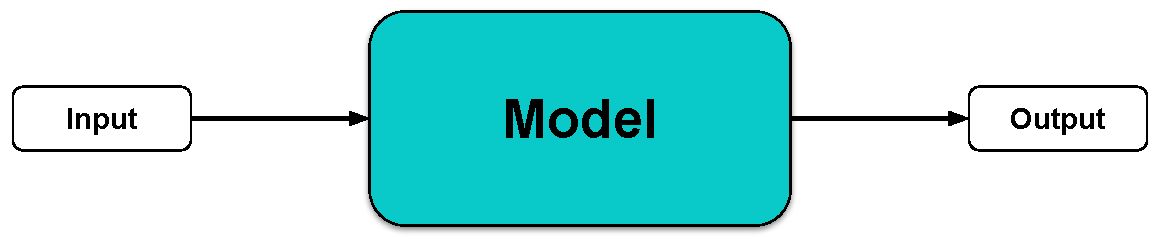
\includegraphics[width=0.75\textwidth]{classical_problem_formulation.pdf}
\caption{Traditional formulation for the story generation task}
\label{fig:classical_problem_formulation}
\end{figure}

In our work instead, we re-formulate the problem in the light of the cycle-consistency framework as shown in \cref{fig:new_problem_formulation}. To this end, given a conditional sequence $\mathbf{x} = (x_1, x_2, \ldots, x_{|\mathbf{x}|})$, a model is first required to translate it into an intermediate sequence $\mathbf{y} = (y_1, y_2, \ldots, y_{|\mathbf{y}|})$ and then another model translates $\mathbf{y}$ into an output (reconstructed) sequence $\hat{\mathbf{x}} = (\hat{x}_1, \hat{x}_2, \ldots, \hat{x}_{|\mathbf{\hat{\mathbf{x}}}|})$. The goal for $\mathbf{x}$ and $\hat{\mathbf{x}}$ is to be as close as possible.

\begin{figure}[ht]
\centering
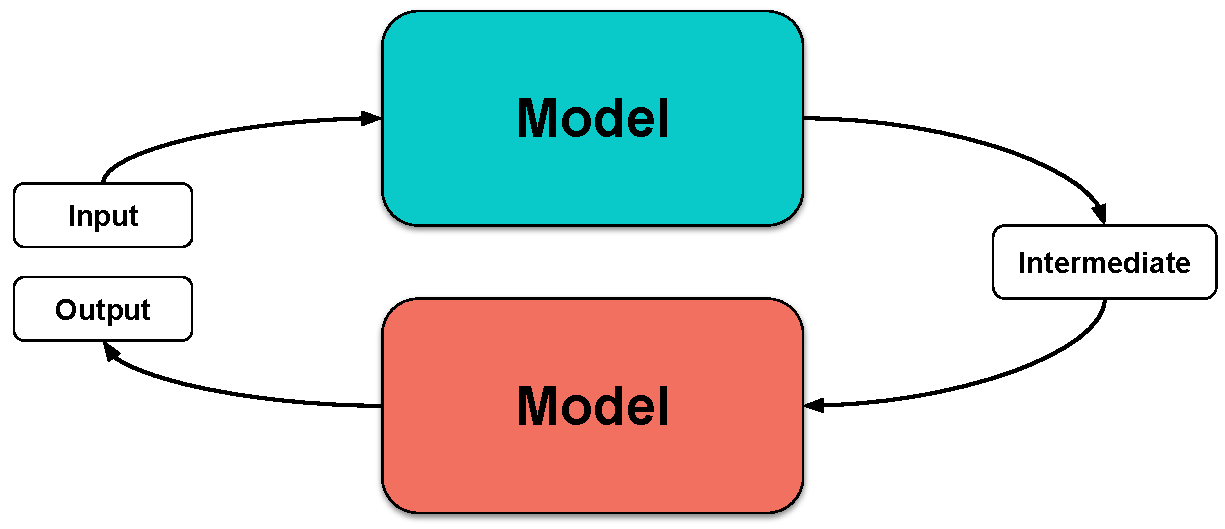
\includegraphics[width=0.75\textwidth]{new_problem_formulation.pdf}
\caption{New formulation for the story generation task}
\label{fig:new_problem_formulation}
\end{figure}

Forcing the original input and its associated reconstruction to be as close as possible leads the models to work together for achieving optimal performance. Indeed, the first model produces text that satisfies a certain task and also conveys the critical information for the other model to operate. The second model instead uses the critical signals in the intermediate text to accurately reconstruct the input. 

Our proposed framework is general enough to consider any two tasks that are considered duals (e.g., translation and back-translation). In this thesis, we specifically study text generation (expansion) and summarization (compression) applied to stories. The expanded text represents a story built from a number of sentences, while the compressed text can be a summary of the story or a title highlighting the theme.


% =================================================================================================

\section{Baseline Architecture}
\label{sec:baseline_arch}

%Since our main task of consideration is story generation, the baseline can be any seq2seq architecture like most of the previous work (\cref{ch:related_work}). However, we base our implementation on BART \citep{lewis2019bart} which is a Transformer-based seq2seq architecture. BART is an encoder-decoder architecture which makes it suitable for text generation tasks since it can both utilize the encoder to access all the input tokens and use the decoder for left-to-right generation. To obtain a baseline to use for future comparison we use one BART model for the expansion task (summary $\mapsto$ story).

Since our main task of consideration is story generation, the baseline can be any seq2seq architecture like most of previous work (\cref{ch:related_work}). The task is then formalized as a conditional generation task (see \cref{fig:baseline_model}) where we want to maximize the output probability distribution
\[ p(\mathbf{y} \mid \mathbf{x}) = \prod_{i=1}^{|\mathbf{y}|} p(y_i \mid \mathbf{y}_{<i}, \mathbf{x})  \]
where $\mathbf{x}$ is the conditional input sequence (summary) and $\mathbf{y}$ is the output sequence (story).

We use BART \citep{lewis2019bart} as our baseline architecture (discussed in \cref{sec:bart_intro}). Using BART gives us the advantage of using the massive knowledge gained from the corpora used to pretrain the model.

\begin{figure}[ht]
\centering
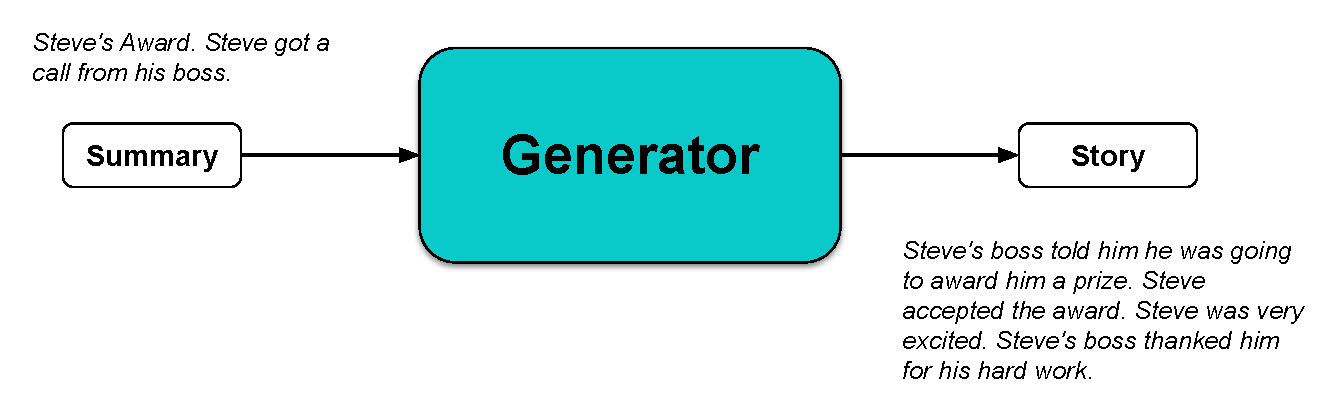
\includegraphics[width=0.75\textwidth]{baseline_model.pdf}
\caption{Baseline seq2seq model}
\label{fig:baseline_model}
\end{figure}


% =================================================================================================

\section{Cycle Architecture}
\label{sec:cycle_arch}

The key concept in this architecture is simplicity. We simply augment the baseline architecture (\cref{sec:baseline_arch}) with another seq2seq model, connect them and let them interact.

The first model performs a conditional generation task where it takes an input sequence $\mathbf{x}$ and maximizes a probability distribution $p(\mathbf{y} \mid \mathbf{x})$ for an intermediate sequence $\mathbf{y}$
\[ p(\mathbf{y} \mid \mathbf{x}) = \prod_{i=1}^{|\mathbf{y}|} p(y_i \mid \mathbf{y}_{<i}, \mathbf{x})  \]

Then the second model samples its input $\mathbf{y}$ from the intermediate probability distribution $\mathbf{y} \sim p(\mathbf{y} \mid \mathbf{x})$ and in turn maximizes a probability distribution $p(\hat{\mathbf{x}} \mid \mathbf{y})$ for an output sequence $\hat{\mathbf{x}}$
\[ p(\hat{\mathbf{x}} \mid \mathbf{y}) = \prod_{i=1}^{|\hat{\mathbf{x}}|} p(\hat{x}_i \mid \hat{\mathbf{x}}_{<i}, \mathbf{y})  \]

Similar to the baseline, we use BART as our architecture for both models. How to sample the intermediate sequence $\mathbf{y}$ from the probability distribution is discussed in the next section (\cref{sec:gumbel_softmax}).

Due to the cyclic nature of the framework, we can set $\mathbf{x}$ and $\hat{\mathbf{x}}$ to be the original and reconstructed summaries respectively, and set $\mathbf{y}$ to the generated story (see \cref{fig:cycle_model_direction_comp}); and also vice versa where $\mathbf{x}$ and $\hat{\mathbf{x}}$ are the original and reconstructed stories respectively, and $\mathbf{y}$ to the generated summary (see \cref{fig:cycle_model_direction_exp}).

\begin{figure}[ht]
    \centering
    \begin{subfigure}[b]{\textwidth}
        \centering
       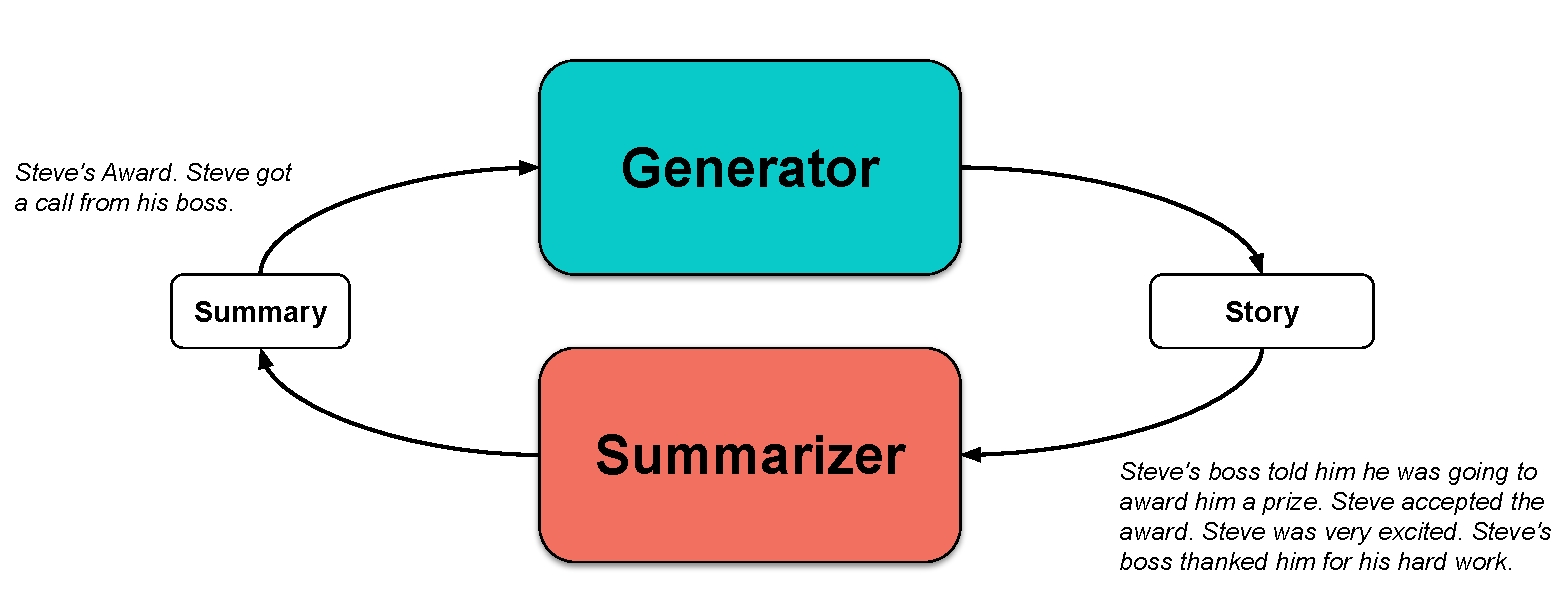
\includegraphics[width=0.75\textwidth]{cycle_model_direction_comp.pdf}
        \caption{First direction: Summary $\rightarrow$ Story $\rightarrow$ Summary}
        \label{fig:cycle_model_direction_comp}
    \end{subfigure}
    \newline \newline
    \begin{subfigure}[b]{\textwidth}
        \centering
       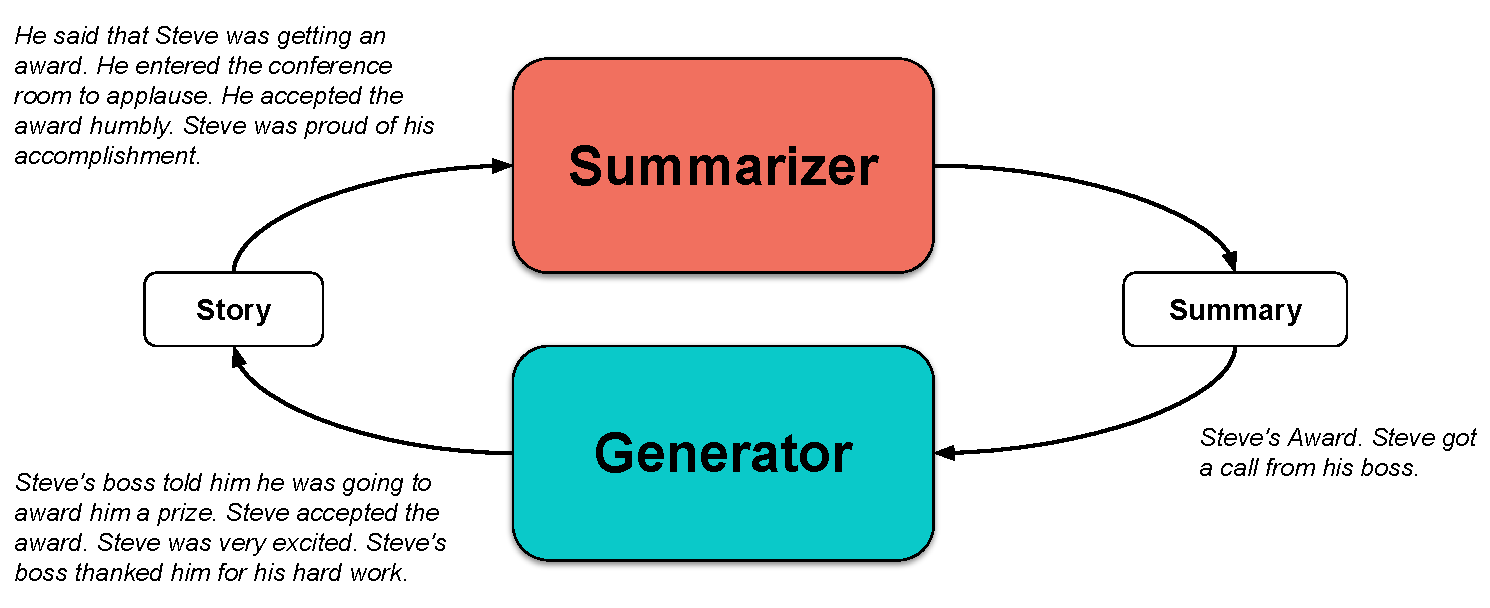
\includegraphics[width=0.75\textwidth]{cycle_model_direction_exp.pdf}
        \caption{Second direction: Story $\rightarrow$ Summary $\rightarrow$ Story}
        \label{fig:cycle_model_direction_exp}
    \end{subfigure}
    \caption{Cyclic nature of the framework}
    \label{fig:cycle_directions}
\end{figure}

An immediate observation from our proposal is the possibility to obtain two good-performing models instead of one; one performs well in expansion (generation), while the other performs well in compression (summarization). However, we only analyze the effect on the expansion process and leave the compression for another study.


% =================================================================================================

\section{Differentiable Sampling}
\label{sec:gumbel_softmax}

To generate the intermediate sequence $\mathbf{y}$, we need to sample the words $(y_1, y_2, \ldots, y_{|\mathbf{y}|})$ from the first model's output categorical distribution: 
\[ p(y_t \mid \mathbf{y}_{<t}, \mathbf{x}) = \text{softmax}(v_t) \]
where $v$ is the unnormalized output (logits) of the model. The simplest method to do so is to use greedy decoding where at each time step $t$ we look for the token with the highest probability:
\[ y_t = \text{argmax} \; p(y \mid \mathbf{y}_{<t}, \mathbf{x}) \]

Since this process uses the argmax operation it is non-differentiable. This results in a training mode similar to \citep{he2016dual} where each model trains separately and they are related only by any information passed through the intermediate text.

To retain the ability to train the whole model using gradient-based optimization where the gradients can backpropagate through both models, we use the Gumbel-softmax (GS) reparameterization trick as an approximation of sampling from categorical distributions \citep{jang2016categorical}. Sampling from the softmax distribution is equivalent to adding to each logit an independent noise factor $\zeta$ from the Gumbel distribution G(0, 1) ($\zeta = -\log(-\log(x_i)), \; x_i \sim Uniform(0, 1) $), and then applying the argmax operation:
\[ y_t \sim \text{softmax}(v_t) \quad \equiv \quad y_t = \text{argmax}(v_t + \zeta) \]

Next, we follow \citep{goyal2017differentiable} in using a soft approximation of the argmax using a peaked softmax function:
\[ e_t = \sum_{i}^{|V|} e(w_i) \; \text{softmax}((v_t + \zeta) / \tau ) \]
where the input for each time step is a weighted sum of all the vocabulary's embeddings and $\tau \in [0, \infty[$ is the temperature used to control the softmax. As $\tau \rightarrow \infty$, the equation approaches a true argmax embedding. Therefore, for a finitely large $\tau$, the obtained embedding is a continuous function of a linear combination of all the embeddings dominated by the most probable word.

By combining the Gumbel-softmax reparameterization trick with the soft argmax, we obtain embeddings that are continuous (thus, differentiable), and maintain the ability to sample from a distribution that adds randomness to make the model robust.

\subsubsection{Straight-Through Estimator}

In our application, we are constrained to sample discrete values (words) from the distribution. As a result, we can not use the continuous approximation shown previously. To this end, we make use of the biased Straight-Through Estimator \citep{bengio2013estimating}. We use the argmax to discretize $\mathbf{y}$ in the forward pass, but in the backward pass, we compute the gradients using the GS soft approximation.


% =================================================================================================

%\section{Semantic Similarity}

%To improve the quality of the generated stories, we impose an extra measurement that focuses on the semantics of the story. The goal for this metric is to motivate the generated story to be as close as possible to the true story \textit{semantically}. A straightforward approach would be to compute the contextualized embeddings of the generated story and label story and maximize the cosine similarity between the vector embeddings. However, we suspect that this approach might create some bias where it forces our model to learn the contextual embedding of the label story.

%Instead our goal is to learn the similarity between the two vectors. First, we finetune a BERT model to our stories dataset. Then during training time, we feed the two stories -- generated and label --  to BERT using the built-in separator token (\texttt{[SEP]}) and use the output \texttt{[CLS]} vector to learn this similarity. We repeat the same process for $k$ negative samples and obtain $k$ \texttt{[CLS]} vectors. We feed the $k$ \texttt{[CLS]} vectors to a linear layer with a pair-wise softmax output that maximizes the score of the correct generated story.

%The semantic similarity module is trained to optimize the following TF-IDF weighted cross-entropy objective function:

%\[ \mathcal{L} = - \sum_{y}^{\mathcal{Y}} \mathcal{P}(x, y) \, \log \mathcal{F}(\{x, y\}; \theta)  \]
%\[ \mathcal{L} = - \sum_{y}^{\mathcal{Y}} \, \log \mathcal{F}(\{x, y\}; \theta)  \]
%\[ \mathcal{L} = - \sum_{i}^{N} \log \mathcal{F}(\{x, y^{+}\}; \theta) + \log(1- \mathcal{F}(\{x, y^{+}\}; \theta)) \]

%where $x$ is the label story, $\mathcal{Y} = \{y^{+}, \bigcup y^{-} \}$ is the set of the generated story and all the negative samples, $\mathcal{F}$ is the probability output of the softmax described above, and $\mathcal{P}$ is a TF-IDF weighting term which calculates the distance between two constructed vectors of the label story and sample story. The constructed vector is a TF-IDF weighted sum of the word embeddings of the story.

%\[ \mathcal{P}(x, y) =  \left\lVert \sum_{i=1}^{N} \frac{\text{IDF}(x_i)}{\sum_{t=1}^{N} \text{IDF}(x_t)} \, e_{i}^{x} \;-\; \sum_{i=1}^{M} \frac{\text{IDF}(y_i)}{\sum_{t=1}^{M} \text{IDF}(y_t)} \, e_{i}^{y} \right\rVert \]



\chapter{Evaluation}
\label{ch:evaluation}


In this section, we overview the datasets we use and what settings/formats they are used in (\cref{sec:datasets}). Then, we discuss the metrics used to evaluate the models (\cref{sec:eval_metrics}). Finally, we report empirical results and comment on them (\cref{sec:experiments}).

\section{Datasets}
\label{sec:datasets}

We use two datasets that are popular and widely used in story generation related works.

\subsection{ROCStories}
\label{sec:roc_stories}

We use ROCStories \cite[ROC]{mostafazadeh2016corpus} to train and evaluate our model. ROC is a dataset of short commonsense stories that focuses on: (1) building causal and temporal relations between commonly encountered day-to-day events that span multiple domains, and (2) high-quality non-fictional events that one could easily relate to, making storytelling models trained on it more believable.

ROC contains 98,161 five-sentence short stories paired with their titles. We use the dataset in two settings shown in \cref{tab:roc-samples}. In the first setting, we use only the title as the input (summary) and the model is required to generate the five sentences. While the second is where we also concatenate the first sentence of the story to the title and the model is asked to predict a story of four sentences. Statistics for the two settings are shown in \cref{tab:roc-statistics}.

\begin{table}[ht]
\centering
\begin{tabular}{p{0.08\linewidth} | p{0.25\linewidth} | p{0.5\linewidth}}
Setting & Summary  & Story \\ \hline
\# 1 & Steve's Award. & Steve got a call from his boss. He said that Steve was getting an award. He entered the conference room to applause. He accepted the award humbly. Steve was proud of his accomplishment. \\ \hline

\# 2 & Steve's Award. Steve got a call from his boss. & He said that Steve was getting an award. He entered the conference room to applause. He accepted the award humbly. Steve was proud of his accomplishment. \\
\end{tabular}
\caption{A sample story from ROC stories%. Top is the first setting with a title-only summary. Bottom is the second setting with title+first sentence summary.
}
\label{tab:roc-samples}
\end{table}

\begin{table}[ht]
\centering
\begin{tabular}{l|rr}

            & Input & Output \\ \hline
Setting \#1 & 5     & 53.35  \\
Setting \#2 & 14.39 & 43.78 \\
\end{tabular}
\caption{Average number of tokens in the input \\ and output for both ROC settings}
\label{tab:roc-statistics}
\end{table}


\subsection{Writing Prompts}
\label{sec:writing_prompts}

Writing Prompts \cite[WP]{fan2018hierarchical} was collected from an online community where users post story prompts and other users are allowed to respond freely with a story that follows the prompt. The prompts vary in terms of length, topic, and level of detail. The stories collected have to be more than 30 words, generally follow the prompt, and avoid profanity.

WP contains 303,358 prompt-story pairs and a prompt can have more than one story. An example is presented in \cref{tab:wp-samples}. Similar to ROC, we explore two settings in WP. The first uses the dataset as-is during training with a maximum story length of 1024 and limits the story to a maximum of 150 tokens at evaluation time. The second limits the story to the first ten sentences (split using NLTK) and uses only a subset of the dataset which is discussed later.


\begin{table}[ht]
\centering
\begin{tabular}{p{0.1\linewidth} | p{0.8\linewidth}}
Summary  & The witch stole his heart, and replaced it with ice. Now he can not love, lest it melts. \\ \hline
Story &
I stare at the retreating figure of the witch who had just cursed me. I feel the cold spread from the lump of ice now in place of my heart. Did she seriously just do this so I can't love again? Love doesn't create actual heat. Don't you understand the laws of thermodynamics? I shout after her slowly fading form. I see a minute shrug as she disappears from my eyeline and give out a weak gurgle as I fall to my knees. As the floor rises to greet my face, it occurs to me that she doesn't much understand the laws of biology either. \\
\end{tabular}
\caption{A sample story from WP}
\label{tab:wp-samples}
\end{table}

\begin{table}[ht]
\centering
\begin{tabular}{l|rr}
            & Input & Output \\ \hline
Setting \#1 & 28.22 & 659.14 \\
Setting \#2 & 28.22 & 164.85 \\
\end{tabular}
\caption{Average number of tokens in the input \\ and output for both WP settings}
\label{tab:wp-statistics}
\end{table}


% =================================================================================================

\section{Evaluation Metrics}
\label{sec:eval_metrics}

We use a combination of automatic evaluation metrics to assess the quality of the generated stories from multiple aspects.

\subsection{Perplexity}
\label{sec:perplexity}

We use perplexity as a method of intrinsic evaluation for the models. For autoregressive language models, perplexity is the inverse of the probability of the dataset normalized by the number of word tokens. Maximizing such probability is equivalent to minimizing the perplexity of the model. Intuitively, the perplexity of an LM is the level of uncertainty when predicting the next token \citep{chip2019evaluation}. For models that use the negative log-likelihood loss, the perplexity can be computed as:
\[ \text{PPL}(X) = \exp \left\{ - \frac{1}{t} \sum_{i}^{t} \log p_{\theta} (x_i \mid \mathbf{x}_{<i})  \right\} \]

Generally, smaller perplexity scores indicate better text fluency.



\subsection{BLEU}
\label{sec:bleu}

Bilingual Evaluation Understudy (BLEU for short) \citep{papineni2002bleu} is a string-matching algorithm that is used for evaluating the quality of translations tasks. BLEU measures the correspondence between machine-generated translations and human-written translations.% Thus a higher BLEU score indicates a better correlation to human performance.
The driving idea is that the closer (more overlapping tokens) the machine translation is to the human's, the better it is.

The BLEU $n$-gram precision $p_n$ is defined over a corpus $\mathcal{C}$ as follows:
\[ p_n = \dfrac
{\sum_{S \in \mathcal{C}} \quad \sum_{n\text{-gram} \in S} \text{Count}_\text{\textit{clip}}(n\text{-gram})}
{\sum_{S' \in \mathcal{C}} \quad \sum_{n\text{-gram} \in S'} \text{Count}(n\text{-gram})}
\]
where $S$ is a sentence or a segment of the corpus, and $\text{Count}_\text{\textit{clip}}$ bounds the count of an $n$-gram to the maximum count found in any single reference for that $n$-gram.

The overall BLEU score is calculated as a geometric mean of the precisions penalized by some brevity penalty to account for short sentences:
\[ \text{BLEU} = \text{BP} \,\cdot\, \exp\left\{ \sum_{i=1}^{N} w_n \log p_n \right\}, \quad
\text{BP} =  \begin{cases}
	\exp\left\{ 1 - \dfrac{|\text{ref}|} { |\text{hyp}| }\right\}, & \text{ if |ref| > |hyp| } \\
	1, & \text{ otherwise } \\
\end{cases}
\]

However, recently BLEU has been criticized for its word-to-word similarity matching making paraphrases or synonyms receive poor scores \citep{callison2006re, cifka2018bleu, mathur2020tangled}. Moreover, texts that contain the right phrases with a wrong/random order can still be considered good. This misleads the overall evaluation of the system. %For this reason, we consider using an evaluation method that takes into account the semantics of the generated text (\cref{sec:bleurt}).


\subsection{Distinctness}
\label{sec:diversity}

Language models tend to generate generic texts that are frequently repeated in text corpora. This is attributed to the objective function used to optimize most LMs -- which is optimizing for the likelihood of outputs given the inputs. Naturally, this leads to neural models picking outputs that maximize the conditional probability which can be a limited set of tokens \citep{li2015diversity}. We follow the work of \citep{li2015diversity} and compute the \textsc{distinct}-$n$ metric to evaluate the diversity of the generated text.

This metric captures the percentage of unique $n$-grams as follows:
\[ \textsc{distinct-}n = \frac{\text{number of unique $n$-grams}}{\text{total number of $n$-grams}} \]

Having a higher distinctness/diversity score would indicate that the model is able to generate novel and interesting text. This is an essential property in storytelling to catch the attention of the reader.


%\subsection{BLEURT}
%\label{sec:bleurt}

%BLEURT \citep{sellam2020bleurt} is a learned metric that uses BERT along with some pretraining signals to learn to evaluate the quality of machine-generated texts. This learnable metric uses BERT to extract contextual embeddings for the input text (conveying semantics) and is trained to optimize multiple regression losses obtained from comparing to BLEU (\cref{sec:bleu}), ROUGE \citep{lin2004rouge}, BERTscore \citep{zhang2019bertscore}, and back-translation.

%BLEURT shows a better correlation to human evaluation and ability to understand semantics -- including paraphrases and synonyms. This makes it applicable to our case where two stories might share the same semantics but have little token overlap.


% =================================================================================================

\section{Experiments}
\label{sec:experiments}

\subsection{Implementation}
\label{sec:implementation}

Our framework can work with any seq2seq model in theory. For our experiments, we use BART as the base block in all variants of the model. We use the Transformers library by Hugging Face \citep{wolf2020transformers} to implement our models. Due to limited resources, we use publicly available pretrained weights of $\text{BART}_\textsc{base}$ \footnote{\url{https://huggingface.co/facebook/bart-base}} to initialize our models. Our models are trained on Tesla P100 and V100 GPUs.

For ROC, the batch size for the baseline model is 64 and for the cycle model 32 with gradient accumulation set to 2 steps. In the first setting, the maximum story length is 110 tokens while for the second it is 90 tokens.

Similarly for WP, the batch size for the baseline is 16 and for the cycle model 8 with gradient accumulation set to 2 steps. In the first setting, the maximum story length is 1024 tokens during training and 150 tokens during evaluation while for the second setting it is 350 tokens.

All models are trained for 20 epochs using the early stopping mechanism that monitors the BLEU score on the validation set with a patience of 5 epochs. At evaluation time, we generate texts using beam search ($n = 5$) on top of nucleus sampling \citep{holtzman2019curious} with $p = 0.9$ and default temperature 1.0. A summary of the hyperparameters can be found in \cref{tab:hyperparameters}.

\begin{table}[ht]
\centering
\begin{tabular}{l|r}
Parameter & Value \\ \hline
\multicolumn{2}{l}{\textbf{ROC}} \\
Baseline batch size & 64 \\
Cycle batch size & 32 \\
Cycle gradient accumulation & 2 steps \\
Max story length (setting \# 1) & 110 tokens \\
Max story length (setting \# 2) & 90 tokens \\ \hline
\multicolumn{2}{l}{\textbf{WP}} \\
Baseline batch size & 16 \\
Cycle batch size & 8 \\
Cycle gradient accumulation & 2 steps \\
Max story length (setting \# 1) & 1024 tokens \\
Max story length (setting \# 2) & 350 tokens \\ \hline
\multicolumn{2}{l}{\textbf{Generation}} \\
Beam size & 5 \\
$p$ & 0.9 \\
Temperature & 1.0 \\ \hline
\end{tabular}
\caption{Hyperparameters used in different models}
\label{tab:hyperparameters}
\end{table}

We test the cycle starting from the two possible endpoints $\text{Cycle}_{\textsc{exp}}$ (Story $\rightarrow$ Summary $\rightarrow$ Story) and vice versa $\text{Cycle}_{\textsc{comp}}$ (Summary $\rightarrow$ Story $\rightarrow$ Summary) -- recall \cref{fig:cycle_directions}. For ROC we report the best out of the two directions (which is $\text{Cycle}_{\textsc{comp}}$) and for WP we report both for reasons outlined in the results section (\cref{sec:wp_results}).

\subsection{Comparison Systems}

In our experiments, we report results for some variants of our models:

\begin{itemize}
\item \textbf{Baseline} -- the baseline model discussed in \cref{sec:baseline_arch}. A BART model that performs a seq2seq task with the summary as input and the story as output.

\item $\textbf{Cycle}_{\textsc{comp}}$ -- the cycle architecture explained in \cref{sec:cycle_arch} where we start with a summary, translate it to a story, and then back into a summary -- recall \cref{fig:cycle_model_direction_comp}.

\item $\textbf{Cycle}_{\textsc{exp}}$ -- the same as $\textbf{Cycle}_{\textsc{comp}}$, but in the other direction where we start with a story, translate it to a summary, and then back into a story  -- recall \cref{fig:cycle_model_direction_exp}.

\item $\textbf{Cycle}_{\textsc{comp}}$-\textbf{GS} -- the same as $\textbf{Cycle}_{\textsc{comp}}$, but the intermediate text is sampled using the Gumbel-softmax reparameterization trick (\cref{sec:gumbel_softmax}) instead of greedy sampling.

\item $\textbf{Cycle}_{\textsc{exp}}$-\textbf{GS} -- the same as $\textbf{Cycle}_{\textsc{exp}}$, but the intermediate text is sampled using the Gumbel-softmax reparameterization trick (\cref{sec:gumbel_softmax}) instead of greedy sampling.
\end{itemize}


We further compare our system with other models from the literature:

\begin{itemize}
\item \textbf{Hierarchical} -- the hierarchical story generation model by \citep{fan2018hierarchical}. They use a ConvS2S LM to generate a premise to guide the story, then they use a seq2seq fusion model to generate the story from the premise.

\item \textbf{H-CVAE} -- the multi-pass CVAE by \citep{yu2020draft}. Their CVAE is built on the seq2seq mechanism with a GRU encoder and a hierarchical decoder that considers global and local semantics. The first CVAE generates a draft of the story from the title, and the second consumes the draft and the title to generate the final story.

\item \textbf{HINT} -- the multi-task model by \citep{guan2021long}. In addition to the LM task, they add a sentence similarity task to learn sentence-level representations and a sentence ordering task to learn discourse-level representations.
\end{itemize}

\subsection{ROC Stories Results}
\label{sec:roc_results}

In \cref{table:roc_1_results}, we show the results for the first setting of ROC stories, which we recall from \cref{tab:roc-samples}, takes as input only the title of the story. B-1 and B-2 stand for \textsc{bleu}-1 and \textsc{bleu}-2 scores, and similarly for D-1 and D-2 with the \textsc{distinct}-$n$ score. PPL stands for perplexity.

\begin{table}[ht]
\centering
\begin{tabular}{l|rr|rr|r}
Model & B-1 $\uparrow$ & B-2 $\uparrow$ & D-1 $\uparrow$ & D-2 $\uparrow$ & PPL $\downarrow$  \\ \hline
Hierarchical & 15.01 & 6.21 & 1.57 & 13.36 & - \\
H-CVAE & 29.39 & 11.02 & 1.99 & 14.82 & - \\ \hline
Baseline & 28.97 & 13.59 & 3.4 & 19.9  & 12.33 \\
Cycle & \textbf{30.19} & \textbf{14.28} & \textbf{3.5} & \textbf{21.2} & 13.919 \\
Cycle-GS & 29.6 & 13.97 & 2.9 & 17.2 & \textbf{11.88}
\end{tabular}
\caption{ROC results for setting \#1}
\label{table:roc_1_results}
\end{table}

Inspecting the results in \cref{table:roc_1_results}, we see the clear advantage of Transformer-based methods over RNN/CNN methods. The baseline model easily achieves comparable performance to the best model (H-CVAE). The cycle framework improves over the baseline in terms of generating more token overlap with reference stories (shown by BLEU score), and more diverse and vivid texts (shown by \textsc{distinct}-n score). We also see the cycle with differentiable sampling improving over the baseline perplexity-wise indicating the ease of modeling test data. We note that we report here the best cycle direction ($\text{Cycle}_{\textsc{comp}}$) since it outperformed the other in most -- if not all -- the metrics.

In \cref{table:roc_2_results}, we show the results for the second setting (see \cref{tab:roc-samples}) of ROC stories, which we recall from \cref{tab:roc-samples}, considers title+first sentence as the input to the model.

\begin{table}[ht]
\centering
\begin{tabular}{l|rr|r|r}
Model & B-1 $\uparrow$ & B-2 $\uparrow$ & D-4 $\uparrow$ & PPL $\downarrow$  \\ \hline
%StyleBART & 33.8 & 17.1 & - & 11.29 \\
HINT & 33.4 & 15.4 & \textbf{69.3} & \textbf{9.2} \\ \hline
Baseline & 35.26 & 18.26 & 58.1 & 11.107 \\
Cycle & \textbf{37.3} & \textbf{20.48} & 67.9 & 11.075 \\
Cycle-GS & 33.79 & 17.1 & 47.6 & 11.743
\end{tabular}
\caption{ROC results for setting \#2}
\label{table:roc_2_results}
\end{table}

As for \cref{table:roc_2_results}, the task in this setting is easier, provided that the model is fed a richer input. Indeed, we see more improvement gaps when it comes to the BLEU score over other SOTA models. Although the cycle improves text diversity over the baseline considerably, there is still room for improvement. As explained earlier this can be attributed to the objective function of optimizing the likelihood of the outputs which generally benefits metrics like BLEU but can hurt text diversity metrics. This can be approached by using the Maximum Mutual Information as suggested by \citep{li2015diversity} to bias to outputs that are specific to the inputs.

For the perplexity, we now see that the vanilla cycle offers a marginal improvement while the differentiable sampling extension is actually not better -- suggesting that the stochasticity introduced by the Gumbel-softmax sampling is unstable and does not always offer better performance. Nevertheless, we expect HINT to have better perplexity since it was pretrained on BookCorpus \citep{zhu2015aligning} before being finetuned on ROC.

%All models score negatively in semantics relatedness to the references (shown by BLEURT). This shows that the extra signals leveraged by the cycle model (and its extension) are not enough to convey semantics and that some extra external signals are needed to guide the model.

\subsection{Writing Prompts Results}
\label{sec:wp_results}

We report the results for the first setting of WP, which we recall from \cref{tab:wp-statistics} trains on stories of 1024 tokens in length, to analyze the effect of long training examples. In this experiment (\cref{table:wp_1_results}), \citep{fan2018hierarchical} report only the perplexity.

\begin{table}[ht]
\centering
\begin{tabular}{l|rr|rr|r}
Model & B-1 $\uparrow$ & B-2 $\uparrow$ & D-1 $\uparrow$ & D-2 $\uparrow$ & PPL $\downarrow$  \\ \hline
Hierarchical & - & - & - & - & 36.56 \\ \hline
Baseline & 28.15 & 12.83 & 1.1 & 6.5  & \textbf{21.24} \\
$\text{Cycle}_{\textsc{exp}}$ & 28.61 & 13.61 & 1.0 & 6.9 & 21.65 \\
$\text{Cycle}_{\textsc{exp}}$-GS & 28.48 & 12.92 & \textbf{1.6} & \textbf{10.3} & 21.97 \\
$\text{Cycle}_{\textsc{comp}}$ & \textbf{31.19} & \textbf{13.8} & 1.0 & 6.0 & 22.243 \\
$\text{Cycle}_{\textsc{comp}}$-GS & 28.37 & 12.92 & 1.4 & 8.9 & 22.04
\end{tabular}
\caption{WP results for setting \#1}
\label{table:wp_1_results}
\end{table}

In \cref{table:wp_1_results}, we discuss the results of training the cycle on longer training examples -- but still testing them on short stories. We can observe how the cycle improved both text overlap and text diversity metrics over the baseline. However, in this case we notice a different behavior where ($\text{Cycle}_{\textsc{comp}}$) has better BLEU scores and ($\text{Cycle}_{\textsc{exp}}$) has better diversity scores. This would indicate that different directions extract different training signals, which can have varying effects on the training procedure. We also notice that unlike for ROC, the Gumbel-softmax extension here has a positive effect on diversity. This might be because that the differentiable sampling procedure works better for longer sequences. The perplexity results are, however, intriguing. It was expected that since the cycle helped improve both overlap and diversity metrics that the perplexity would follow -- which is not the case. The reason behind this is not clear and needs more investigation.

In \cref{table:wp_2_results}, we show the results for the second setting for WP, which we recall from \cref{tab:wp-statistics}, limits the story to the first ten sentences.

\begin{table}[ht]
\centering
\begin{tabular}{l|rr|r|r}
Model & B-1 $\uparrow$ & B-2 $\uparrow$ & D-4 $\uparrow$ & PPL $\downarrow$  \\ \hline
HINT & 22.4 & 8.4 & 31.3 & 32.73 \\ \hline

 & \multicolumn{4}{c}{\textbf{30K stories}} \\ \hline
Baseline & 23.92 & 9.68 & 48.0  & 43.02 \\
$\text{Cycle}_{\textsc{exp}}$ & 22.41 & 8.9 & 61.4 & 43.25 \\
$\text{Cycle}_{\textsc{comp}}$ & 23.0 & 9.33 & 47.4 & 43.16 \\ \hline

 & \multicolumn{4}{c}{\textbf{100K stories}} \\ \hline
Baseline & 26.22 & 10.52 & 32.7  & \textbf{40.05} \\
$\text{Cycle}_{\textsc{exp}}$ & 27.3 & 10.84 & \textbf{47.0} & 42.51 \\
$\text{Cycle}_{\textsc{exp}}$-GS & 28.39 & 11.3 & 45.4 & 42.57 \\
$\text{Cycle}_{\textsc{comp}}$ & \textbf{29.63} & \textbf{11.79} & 40.8 & 42.22 \\
$\text{Cycle}_{\textsc{comp}}$-GS & 26.89 & 10.69 & 45.4 & 44.06
\end{tabular}
\caption{WP results for setting \#2}
\label{table:wp_2_results}
\end{table}

In the second setup (\cref{table:wp_2_results}) we follow the parameters set by \citep{guan2021long} to obtain comparable results. We use $\sim$30K stories to finetune our models, however, we directly notice that the models are overfitting the training data. We hypothesize that it is difficult for the model to train on longer sentences with fewer instances (compared to ROC). Additionally, \citep{guan2021long} pretrained their model on BookCorpus before finetuning it on the $\sim$30K (10\%) stories from WP. Due to these reasons, we increase our dataset to use $\sim$100K (33\%) random stories from WP and still follow the rest of the parameters.

We obtain similar observations where ($\text{Cycle}_{\textsc{comp}}$) has better BLEU scores and ($\text{Cycle}_{\textsc{exp}}$) has better diversity scores. And with similar perplexity behavior, we attribute these findings to the bigger size of the dataset in terms of both summary and story lengths (compared to ROC). It would appear that in $\text{Cycle}_{\textsc{comp}}$ the story generators tries to produce as much token overlap as possible so that the summarizer can successfully reconstruct the summary again. However, when it is used in the other direction, the story generator has more freedom over the story and generates stories with more vivid text.

%The results obtained by semantics metric (BLEURT) would confirm the findings in ROC that extra signals are required to help the models generate more semantically relevant stories. We notice that since the stories are bigger, the semantic divergence from the references is also more than that of ROC. This would attest to the fact that there are no implied semantic signals learned by the cycle framework solely.


% =================================================================================================

\section{Qualitative Analysis}

In this section, we study some cases of generated stories by different models. In the first example (\cref{tab:comp-sample-1}), we see a sample from ROC -- with the gold summary (input), gold story (output), and generated stories by the baseline and cycle models.

\begin{table}[h]
\centering
\begin{tabular}{p{0.2\linewidth} | p{0.7\linewidth}}
Gold Summary (input)  & Steve's Award. Steve got a call from his boss. \\ \hline
Gold Story & He said that Steve was getting an award. He entered the conference room to applause. He accepted the award humbly. Steve was proud of his accomplishment. \\ \hline
Generated Story (Baseline) & He was given a big award for his hard work. Steve was so proud of himself. \textcolor{red}{\textit{He took the award home and presented it to his boss.}} Steve's boss was very proud of him. \\ \hline
Generated Story (Cycle) & Steve's boss told him he was going to award him a prize. Steve accepted the award. Steve was very excited. Steve's boss thanked him for his hard work.
\end{tabular}
\caption{Generated stories by different models for the same input (1)}
\label{tab:comp-sample-1}
\end{table}

For the story generated by the baseline, we see a case of reverse semantics where the employee gives an award to his boss. This is not the intended meaning (seen in the gold story). We see that the cycle could correctly capture the semantics in this example and produce a coherent story.

In the second example (\cref{tab:comp-sample-2}), we see that the two cycle directions produce semantically different results. The $\text{Cycle}_{\textsc{exp}}$ model failed to understand the global semantics of the story, thus producing an irrelevant story. This problem is not propagated by the other cycle model, confirming that the signals extracted by the two directions are different.

\begin{table}[h]
\centering
\begin{tabular}{p{0.2\linewidth} | p{0.7\linewidth}}
Gold Summary (input)  & Nicole's Boyfriend Nicole did not have a serious boyfriend. \\ \hline
Gold Story & She went on many dates but was not committed. She was at a bar one night and met a man she was interested in. They began dating. Nicole just got engaged to be married. \\ \hline
Generated Story ($\text{Cycle}_{\textsc{exp}}$) & Nicole did not have a boyfriend. Nicole decided to get a job. Nicole applied for a job at a restaurant. Nicole got a job as a waitress. \\ \hline
Generated Story ($\text{Cycle}_{\textsc{comp}}$) & Nicole decided to go out with her friends. Nicole met a guy at a bar. Nicole fell in love with the guy. Nicole and her boyfriend are now married.
\end{tabular}
\caption{Generated stories by different models for the same input (2)}
\label{tab:comp-sample-2}
\end{table}

In the third example (\cref{tab:comp-sample-3}), we notice that none of the models correctly understand the meaning of the word ``wake''. The intended meaning is ``a vigil held over a corpse the night before burial'' \footnote{All definitions in this paragraph are according to WordNet.} which means the death of someone and the feeling of sadness for the relatives and close people. Instead, we see two of the models understood the verbal meaning of ``to stop sleeping'', and the other could not convey the sentiment correctly. We argue that this is a hard example and more relevant information needed to be passed to the models.

\begin{table}[h]
\centering
\begin{tabular}{p{0.2\linewidth} | p{0.7\linewidth}}
Gold Summary (input)  & Wake. Anette put on a wake for her grandmother. \\ \hline
Gold Story & Her grandmother had passed away the previous week. Anette put together a playlist of her grandma's favorite songs. They were all upbeat rock \& roll tunes. Anette cried as she danced. \\ \hline
Generated Story (Baseline) & \textcolor{red}{\textit{She was very nervous to wake her grandmother.}} But she was determined to make her grandmother feel better. She put on her grandmother's favorite song. Her grandmother was so happy to see Anette again! \\ \hline
Generated Story ($\text{Cycle}_{\textsc{exp}}$) & She put the wake in her grandmother's bedroom. Anette went to the kitchen to make breakfast. She made pancakes for her grandmother. \textcolor{red}{\textit{Her grandmother thanked Anette for the wake.}} \\ \hline
Generated Story ($\text{Cycle}_{\textsc{comp}}$) & She was very nervous about it. \textcolor{red}{\textit{But when she woke up, she was relieved.}} Her grandmother had passed away. Anette was glad she had put on a wake for her.
\end{tabular}
\caption{Generated stories by different models for the same input (3)}
\label{tab:comp-sample-3}
\end{table}



\chapter{Conclusion}
\label{ch:conclusion}

In this thesis, we present the cycle-consistency framework to the story generation task. To the best of our knowledge, this was the first attempt to do so. We provide a clear and intuitive new formulation for the story generation problem, that is easily understood and extendable.

Previously, the problem was perceived as a conditional generation problem where given an input sequence (summary) the model was required to output a story. Instead, we propose to generate first an intermediate text that is further improved by signals obtained from an input-reconstruction task, through the use of two models.

In addition, we experiment with two sampling methods; greedy sampling and Gumbel-softmax sampling. With greedy sampling, the two models are trained separately and combined only by the intermediate text, while using Gumbel-softmax sampling, makes the whole cycle fully differentiable which allows for better gradient-based optimization.

We prove that this formalization improves over others in several metrics. We show that the cycle model can extract meaningful signals that help with generating text with higher diversity and overlap with reference texts.

As future work, we intend to experiment with new external signals to guide the cycle model. We plan on introducing a semantic similarity signal which serves the purpose of making the generated story more semantically related to the reference. We also plan on using commonsense knowledge bases to improve the logical coherency of the generated text.


\backmatter

% bibliography
\cleardoublepage
\phantomsection
\addcontentsline{toc}{chapter}{\bibname}
%\bibliographystyle{sapthesis} % BibTeX style
%\bibliographystyle{abbrvnat} % BibTeX style
\bibliographystyle{styles/acl_natbib}
\bibliography{references} % BibTeX database without .bib extension


\end{document}
